% ****** rbf.tex ******
% Este archivo provee el formato para la Revista Boliviana de Fisica, RBF.
\documentclass{rbf}
\usepackage{amsmath}
%\usepackage{natbib}
\usepackage[utf8]{inputenc}
\usepackage{subfig}

\begin{document}
        
\title{Bitcoin}

\author{Brandom Chicharito\marca{*}}
\afil{Carrera de Física, Universidad Mayor de San Andrés}%
\alpie{*}{brandoum@fiumsa.edu.bo}

\author{J. C. Vargas\marca{\dag}}
\afil{Fellow Researcher, Bitcoin Research}
\alpie{\dag}{jp.cr3spo@pm.me}
 
\author{Alfredo Carrillo Mendoza\marca{\ddag}}
\afil{Fellow Researcher, Bitcoin Research}
\alpie{\ddag}{acarrillom@proton.me}% Las lineas se cortan automaticamente o puede obligarse esto con

\begin{abstract}
\Resumen
En este artículo se presenta los resultados de tres metodologías diferentes en las que se aplicó una simulación Monte Carlo para estimar el valor de $\pi$: el método de comparación de áreas, el método propuesto por Buffon y la extensión de Laplace al método de Buffon. Se estudió con detalle el resultado no determinista de las simulaciones y se demostró que cumplen con los teoremas fundamentales de la probabilidad. Los tres casos se desarrollaron en un lenguaje de programación de alto nivel: Python, junto con la librería Numpy que le otorga un performance optimizado.

\descriptores{Simulación, Monte Carlo, $\pi$, Buffon, Buffon-Laplace, Python, Numpy}


\Abstract
This article represents the result of three different metodologies for estimate the $\pi$ value with Monte Carlo's simulation: the comparition area's method, the method proposed by Buffon and the Laplace's extention. The non-deterministic result of the simulations was studied in detail and it was shown that they comply with the fundamental theorems of probability. The three cases had been developed in  Python (high level language) and Numpy library which give it an optimized performance. 

\keywords{Simulation, Monte Carlo, $\pi$, Buffon, Buffon-Laplace, Python, Numpy}
\end{abstract}

\maketitle

%%%%%%%%%%%%%%%%%%%%%%%%%%%
%   INTRODUCCION
%%%%%%%%%%%%%%%%%%%%%%%%%%%



\section{Introducción}

Bitcoin es el nombre de la primera solución tecnológica descentralizada en la historia de la humanidad. Se compone de computadoras que corren un software desarrollado bajo el paradigma FOSS (Free and y Open Source Software), llamado «cliente Bitcoin-Core», disponible en distintos sistemas operativos (Windows, Linux y Mac) con requisitos mínimos de hardware capaz de correr desde un Raspberry en adelante. Se denomina descentralizado pues la red no tiene ni un solo punto (o nodo) de confianza, lo que significa que todos los nodos tienen la misma prioridad en la validación de información en la red. 


La palabra 'Bitcoin' se registra por primera vez el 18 de agosto de 2008 al reservarse el dominio de Internet "www.bitcoin.org". Días después se detalla su propuesta de funcionamiento en un White Paper publicado en Internet bajo el pseudónimo de 'Satoshi Nakamoto', en un foro de discusión sobre criptografía el 31 de octubre de 2008 con el título "Bitcoin: A Peer-to-Peer Electronic Cash System". 

Bitcoin tiene una raíz etimologíca compuesta por dos palabras: "bit" que es la unidad mínima de informacion digital y "coin" una palabra en ingles para referirse a «moneda» que es un medio de intercambio indirecto de bienes económicos. Bitcoin busca crear un sistema económico nuevo cuyo título del paper expresa precisamente, traduciendo al español: «Efectivo electrónico transmitido de punto a punto». No se propuso para ser el primer dinero digital (en 2008 la banca digital ya existía) sino ser el primer sistema monetario digital que tenga propiedades que se comparen al dinero en efectivo, como ser: la  portabilidad, la privacidad más no anonimidad (una transacción personal no recopila datos), la fácil verificación de autenticidad (sellos acuñados en monedas o marcas de seguridad en billetes),  la disposición (liquidez), etc. pero principalmente destacamos una propiedad que únicamente emerge en esta red: Ser "Permisionless", que significa 'no necesitar el permiso' de ningún punto o actor en la red para efectuar una transacción. Esta caracteristica implica eliminar todo punto de confianza dando la capacidad de auditar a cualquier componente de la red (código, base de datos, firmas digitales, etc) en cualquier momento. Esta propiedad y sus efectos surgen al mantener un consenso sobre los 'estados' denominados UTXOs de la red. Esta información común y compartida por toda la red se almacena en una base de datos llamada Blockchain. Se divide en trozos 'encadenados' uno tras otro en bloques de información del tamaño de 1 MB. Cada bloque nuevo actualiza estos 'estados' aportando nueva información compartida por toda la red.

Esta nueva actualización de estados es común en toda la red mediante el protocolo de consenso. Al tener todos los participantes el mismo rango en la red ninguno tiene el poder de imponer su historial e independientemente de si hay un participante malicioso todo el conjunto debe mantener la misma información. Este problema es conocido al estudiar la información en sistemas distribuidos como 'El problema de los generales bizantinos' \cite{bizantinos}. Bitcoin hace uso de un protocolo de consenso de red llamado Proof of Work o Prueba de Trabajo que consiste en la necesidad de reunir una cantidad de trabajo en el mundo físico (en forma de energía eléctrica) para producir un nuevo estado de información digital común en el ciberespacio. Esta prueba de trabajo que se solicita es variable y depende del tamaño y poder computacional de toda la red.

La energía eléctrica necesaria para el cambio de estados UTXO es un respaldo de seguridad para la inmutabilidad 
de la información compartida en el ciberespacio. La información que contiene el blockchain es computada por toda la red. Es por esta razón que la red Bitcoin se compara a una sola máquina universal de estados turing completo de escala global, una especie de superordenador con la capacidad de realizar la verificación mediante computo y mantenerlo inmutable en la red.


En la siguiente sección II explicamos como funciona internamente el sistema rígido y predecible de reglas que expresa el código fuente de Bitcoin-Core.  Para la seccion III estudiamos la red con los datos auditados propiamente y finalmente en la sección IV exponemos los resultados.


\section{Diseño de la Red}

Bitcoin se diseño bajo un cierto esquema de principios e incentivos que mantienen segura a la red. Mientras una sola entidad no contenga la mayoría del poder computacional de la red, está es segura. 

El funcionamiento sobre los incentivos esta expresado en el código de Bitcoin Core, cuyo punto fuerte es la limitación de la red para emitir un activo que funge para los intercambios de la red: 'bitcoin'. Cabe notar la diferencia en la nomenclatura radica en el uso de la mayúscula para diferenciar la red Bitcoin del activo subyacente de esta, bitcoin. Este activo se denomida como 'real e intangible' en el sentido que no tiene un carácter contractual (no tiene una obligación de pago ni derecho de cobro) y que al ser digital no guarda relación física en nuestro medioambiente físico (tierra agua aire) pero tiene una existencia irreproducible en un nuevo ámbito de interacción humana: el ciberespacio. 

El activo de bitcoin hace una definición nueva del concepto de propiedad privada al hacerla absoluta. Esta propiedad es inexistente en el campo físico pues cualquier recurso puede ser tomado por la fuerza o su proyección, sin embargo, bitcoin se puede considerar con un landing digital que no puede ser violado de ninguna manera por ningún tipo de fuerza o proyección de poder, al fundamentar su seguridad digital en la producción de energía eléctrica (medida en Julios) del mundo físico. Se necesita de una cantidad colosal de energía eléctrica para generar el cambio en un bloque de la red. 

El sistema de incentivos que mantiene la seguridad de la red toma como punto central la escasez digital. La cantidad de bitcoin que puede ser emitido es finito y calculable en todo momento siendo cercano a los 21 millones de unidades en total. Esto lo logra mediante código de computadora que no puede  cambiado por algún actor de red pues implicaría que todos (el 100\% de la red) la asuma voluntariamente. 

La regla de emisión de bitcoin se da mediante el siguiente esquema:

1. Cada bloque generado por cualquier componente de la red debe demostrar una cantidad de trabajo computacional (que consume energía eléctrica).

2. Como recompensa al gasto de energía el sistema entrega un incentivo de nuevo bitcoin, que inicia en 50 btc.

3. Cada 210 000 bloques este incentivo se ajusta reduciendose a la mitad. Cada bitcoin puede ser dividio en partes más pequeñas hasta un factor de 100 millones, unidad que se denomina satoshis o sats. Este evento donde la emisión se reduce a la mitad se denomina HALVING.

4. La división a la mitad del incentivo se detiene cuando llega a la 100 millonesima parte (o lo que es 1 sat), terminando la emisión de nuevos bitcoins en la red.

5. La salida temporal de nuevos bloques es altamente variable con un valor esperado de 10 minutos. Si se hace una cuenta rápida cada 210 mil bloques representa cerca de 4 años. 

6. Una cuenta rápida muestra que todo el bitcoin existente se emitirá hasta el año 2140. Luego de este el beneficio para seguir generando nuevos bloques será unicamente la comisión que los usuarios decidan dar al productor, recirculando la cantidad fija de bitcoin existentes.


INSERTAR GRAFICO DE EMISION Y EXPLICAR CADA PERIODO COMO HALVING






\section{Como se pensó la red}

La red se pensó para tener un número  finito de cuentas pero humanamente infinito, el número de cuentas se pensó para que cualquiera pueda tener una cuenta pensando solo en un número de 256 cifras binarias(uno o cero), equivalente a un número de 77 cifras, a este número le vamos a llamar contraseña privada,la cantidad máxima de números posibles con 256 ceros y unos es: 

\begin{equation}
    2^{256} -1= N_{max}
\end{equation}


$N_{max}$ representa el límite superior de cuentas posibles, y es tan inmenso que incluso si alguien creara 10 cuentas por segundo, llevaría más de un siglo para agotar todas las posibles cuentas. Debido a la extraordinaria magnitud de este número, si una persona eligiera un número al azar, la probabilidad de que otra persona elija el mismo es extremadamente remota, casi inexistente.
\\
Tras elegir un número este pasa a ser transformado mediante la criptografía de curva elíptica por sus siglas en ingles(ECC), la curva que se usa en la red bitcoin es secp256k1 (Standards of Efficient Cryptography), el número 256 indica la longitud en bits del campo primo p , el termino k1 indica que es la primera curva de este tipo recomendada por el SECG (Standards of Efficient Cryptography Group),que corresponde a la ecuación:
\\
\begin{equation}
    \centering
    y^{2} = X^{3}+7(mod \quad p)
\end{equation}
\\
Donde la operación mod(p) garantiza que todos los cálculos se realizan dentro de un campo finito que es conjunto finito de elementos sobre el cual se pueden realizar operaciones aritméticas básicas, p es un número primo grande.
\\
\begin{figure} [h]
  \subfloat[$y^{2} = X^{3}+7$]{\includegraphics[width=0.2\textwidth]{ECC_continuo.png}}
  \hspace{1cm}
  \subfloat[$y^{2} = X^{3}+7(mod p)$]{\includegraphics[width=0.2\textwidth]{ECC_discreto.png}}   
    
 \caption{Curva elíptica $y^{2} = X^{3}+7$  a) campo continuo  b)  campo finito }
 
\end{figure}
\\
El número que nosotros elegimos como clave privada se multiplica por un número generador G(x,y), y se procede a calcular su suma de la siguiente manera, si nosotros elegimos el número n , este se calcula como n*G como la suma de G así mismo n veces. El número generador en base hexadecimal y en base decimal que se utiliza es :
\\
{\small
G=(0x79BE667EF9DCBBAC55A06295CE870B0
\\7029BFCDB2DCE28D959F2815B16F81798,
\\0x483ADA7726A3C4655DA4FBFC0E1108A
8FD17B448A68554199C47D08FFB10D4B8).\\

}
que en base decimal es:
{\small
G=(5506626302227734366957871889516853432625
0603453777572733226205679730040724416, 
\\3267051002075881697808308513050704318447
1273380659243275938904335757337482424).\\

}

Dicho algoritmo transforma un número en una salida que no se puede predecir y además es irreversible, es decir no se pueden obtener las entradas(clave privada) conociendo la salida y si nosotros solo tuviéramos acceso a esas salidas no podríamos decir que número produce dicha salida.

Por ultimo necesitamos una dirección publica, la cual se puede obtener a través del algoritmo SHA-256 (Secure Hash Algorithm 256 bits), el cual es un algoritmo que transforma cualquier conjunto de datos en una cadena de salida fija de 256 bits es decir 64 caracteres a esta salida s la denomina Hash.
\\ 
Es importante distinguir entre estos dos conceptos en el contexto de Bitcoin: SHA-256 es utilizado para operaciones Hash, mientras que la criptografía de curva elíptica se utiliza para la generación y verificación de claves.
\\
También se debe entender como funcionan los nodos de la red, al igual que cualquier persona puede crearse una clave privada y una dirección, cualquier persona es capaz de conectar su nodo a la red, las acciones que este nodo puede hacer dentro la red son: 
\\
\textbf{Validación de bloques:} Los nodos pueden verificar y validar todas las transacciones que se envían a la red, verifican que las firmas digitales sean validas  y que los fondos no se gasten dos veces
\\
\textbf{Mantenimiento del libro mayor:} Cada nodo mantiene una copia de la cadena de bloques y esta información es publica.
\\
\textbf{Difusión de información:} Los nodos trasmiten nuevas transacciones y bloques validados a otros nodos, esto mantiene la red actualizada.
\\
\textbf{Acceso a la red:} Cada nodo permite interactuar con la red y consultar los estados de la red, estos estados se verifican a través de los UTXO (Unspent Transaction Output), que representan la parte no gastada de una transacción, cada entrada de una transacción se dirige a un UTXO y cada uno de estos tiene una cantidad de Bitcoin asociada y se puede usar en una nueva transacción, estos UTXO's son esenciales para el seguimiento y seguridad de la red, así se verifican que las entradas de una transacción apunten a un UTXO valido y que la cantidad de Bitcoin gastada no exceda los UTXO de entrada, de esta manera se garantiza que no se puedan crear Bitcoin de la nada y que estos no se gasten dos veces. 
\\
\textbf{Participación en la minería:} Un nodo se puede configurar para que participe en la minería de Bitcoin, estos nodos se conocen como mineros, esto implica competir para agregar nuevos bloques a la cadena, para lograr esto deben resolver pruebas de Hash  y de tener éxito se obtiene una recompensa en forma de monedas digitales Bitcoin.
\\
\section{Nodos configurados como mineros}
Los nodos reciben múltiples solicitudes de transacciones, las cuales, después de ser validadas por los nodos, se almacenan en una memoria temporal y pública conocida como mempool o pool de transacciones sin confirmar. Cuando un minero decide crear un nuevo bloque, selecciona ciertas transacciones de esta memoria, generalmente priorizando aquellas que ofrecen una comisión más alta. A esta comisión se le denomina "fee de transacción", donde "fee" es un término inglés que significa "comisión".
\\
Posteriormente se procede a la  resolución de las pruebas de Hash que se realizan empezando por ver la dificultad de la red, esta dificultad es una condición que impone la red y consiste en que el Hash que se saque al siguiente bloque debe comenzar por una cantidad de ceros impuesta por la red, para poder crear un Hash que tenga la cantidad de ceros impuesta por la red se debe agregar al encabezado del bloque un número de 32 bits conocido como 'nonce' por su significado en ingles(number used once), este valor se va cambiando en el bloque a medida que se le saca el Hash una y otra vez  hasta que produzca un Hash que cumpla el número de ceros de la red, puede darse el caso de que al pasar por todos lo valores posibles del nonce $2^{32}-1$, no se produzca ningún Hash con la cantidad de ceros necesarios, en ese caso el minero saca algunas transacciones de su bloque y adhiere otras de la memoria mempool y comienza nuevamente a realizar las pruebas de Hash, en caso de que este logre crear un bloque que cumpla con la dificultad de la red este bloque contendrá la información de las transacciones y además se obtendrá una recompensa por el minado de este bloque, la recompensa se llama Coinbase y el minero agrega estas monedas recompensa del Coinbase a una dirección(generalmente la dirección del minero), posteriormente este nuevo bloque pasa a ser verificado y difundido en la red a través de los nodos.
\\
Puede darse el caso que dos nodos en distintas partes del mundo logren crear un bloque valido para la red, en ese caso se sigue la regla de la cadena mas larga y el bloque que se queda en la red sera el bloque que logre ser validado por mas nodos, y la red se quedara con el bloque sobre el que se escriba otro bloque valido.
\\
Visto de esta manera es erróneo pensar en la prueba de Hash como trabajo realizado o como la resolución de rompecabezas criptográficos o como el calculo de algún problema, pues la manera en la que se crean los nuevos bloques en la cadena esta fuertemente ligado al azar, es decir tener mas poder computacional te asegura realizar mas Hashe's por segundo pero no te garantiza el minado del bloque y al no ser poder de calculo su coste es netamente el precio de la energía.
\\
La red ajusta la dificultad en función al tiempo de minado de los bloques de manera que se trate de tener un promedio en el tiempo de llegada entre bloques de 10 minutos este ajuste ocurre cada 2016 bloques que corresponde a 14 días aproximadamente.

\begin{figure} [h]
  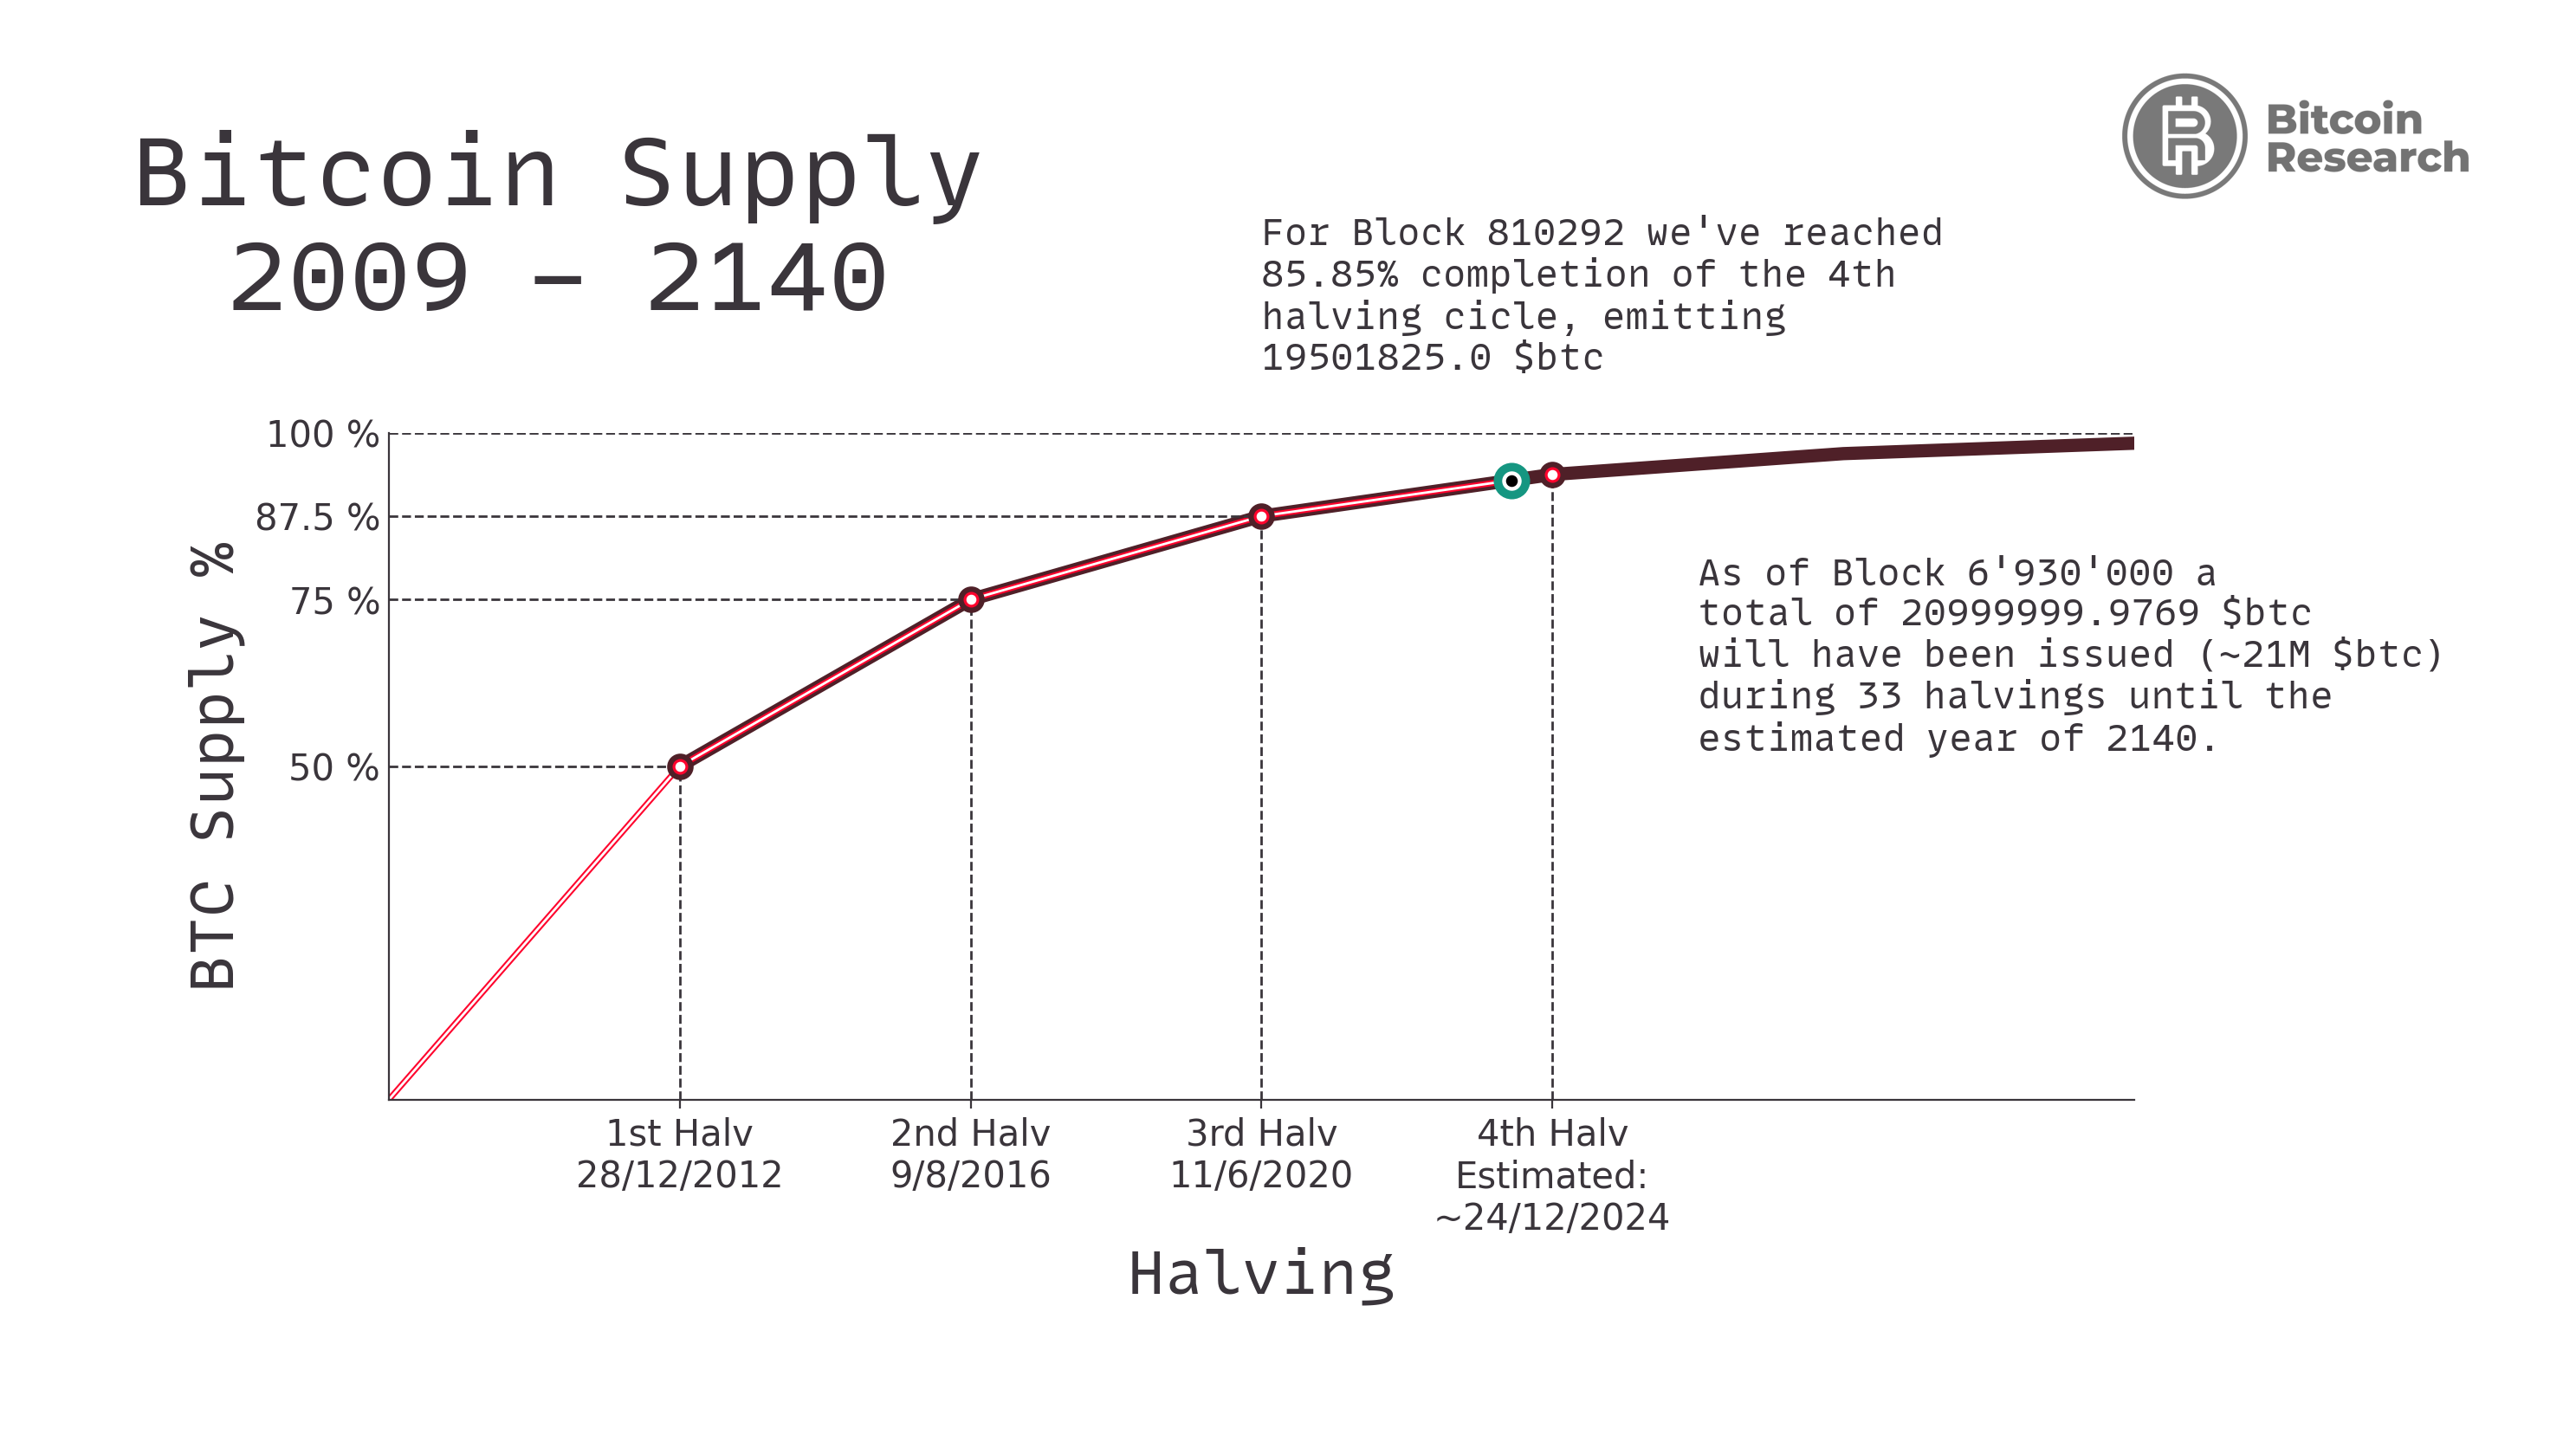
\includegraphics[width=0.5\textwidth]{supply_btc_estilo_blanco.png}
    
 \caption{Cantidad de BTC minados.-Al igual que la red ajusta la dificultad también ajusta la recompensa del Coinbase cada 210000 bloques, a este evento se lo denomina Halving, y reduce la recompensa por minado de los bloques a la mitad, la red empezó en 50BTC por minado de Bloque. }


\end{figure}


\section{Análisis de la red}
Para realizar un análisis histórico de la red, se tuvo acceso a un nodo dentro de la red y mediante  este se obtuvieron los datos de los bloques de la red.

\begin{figure} [h]
  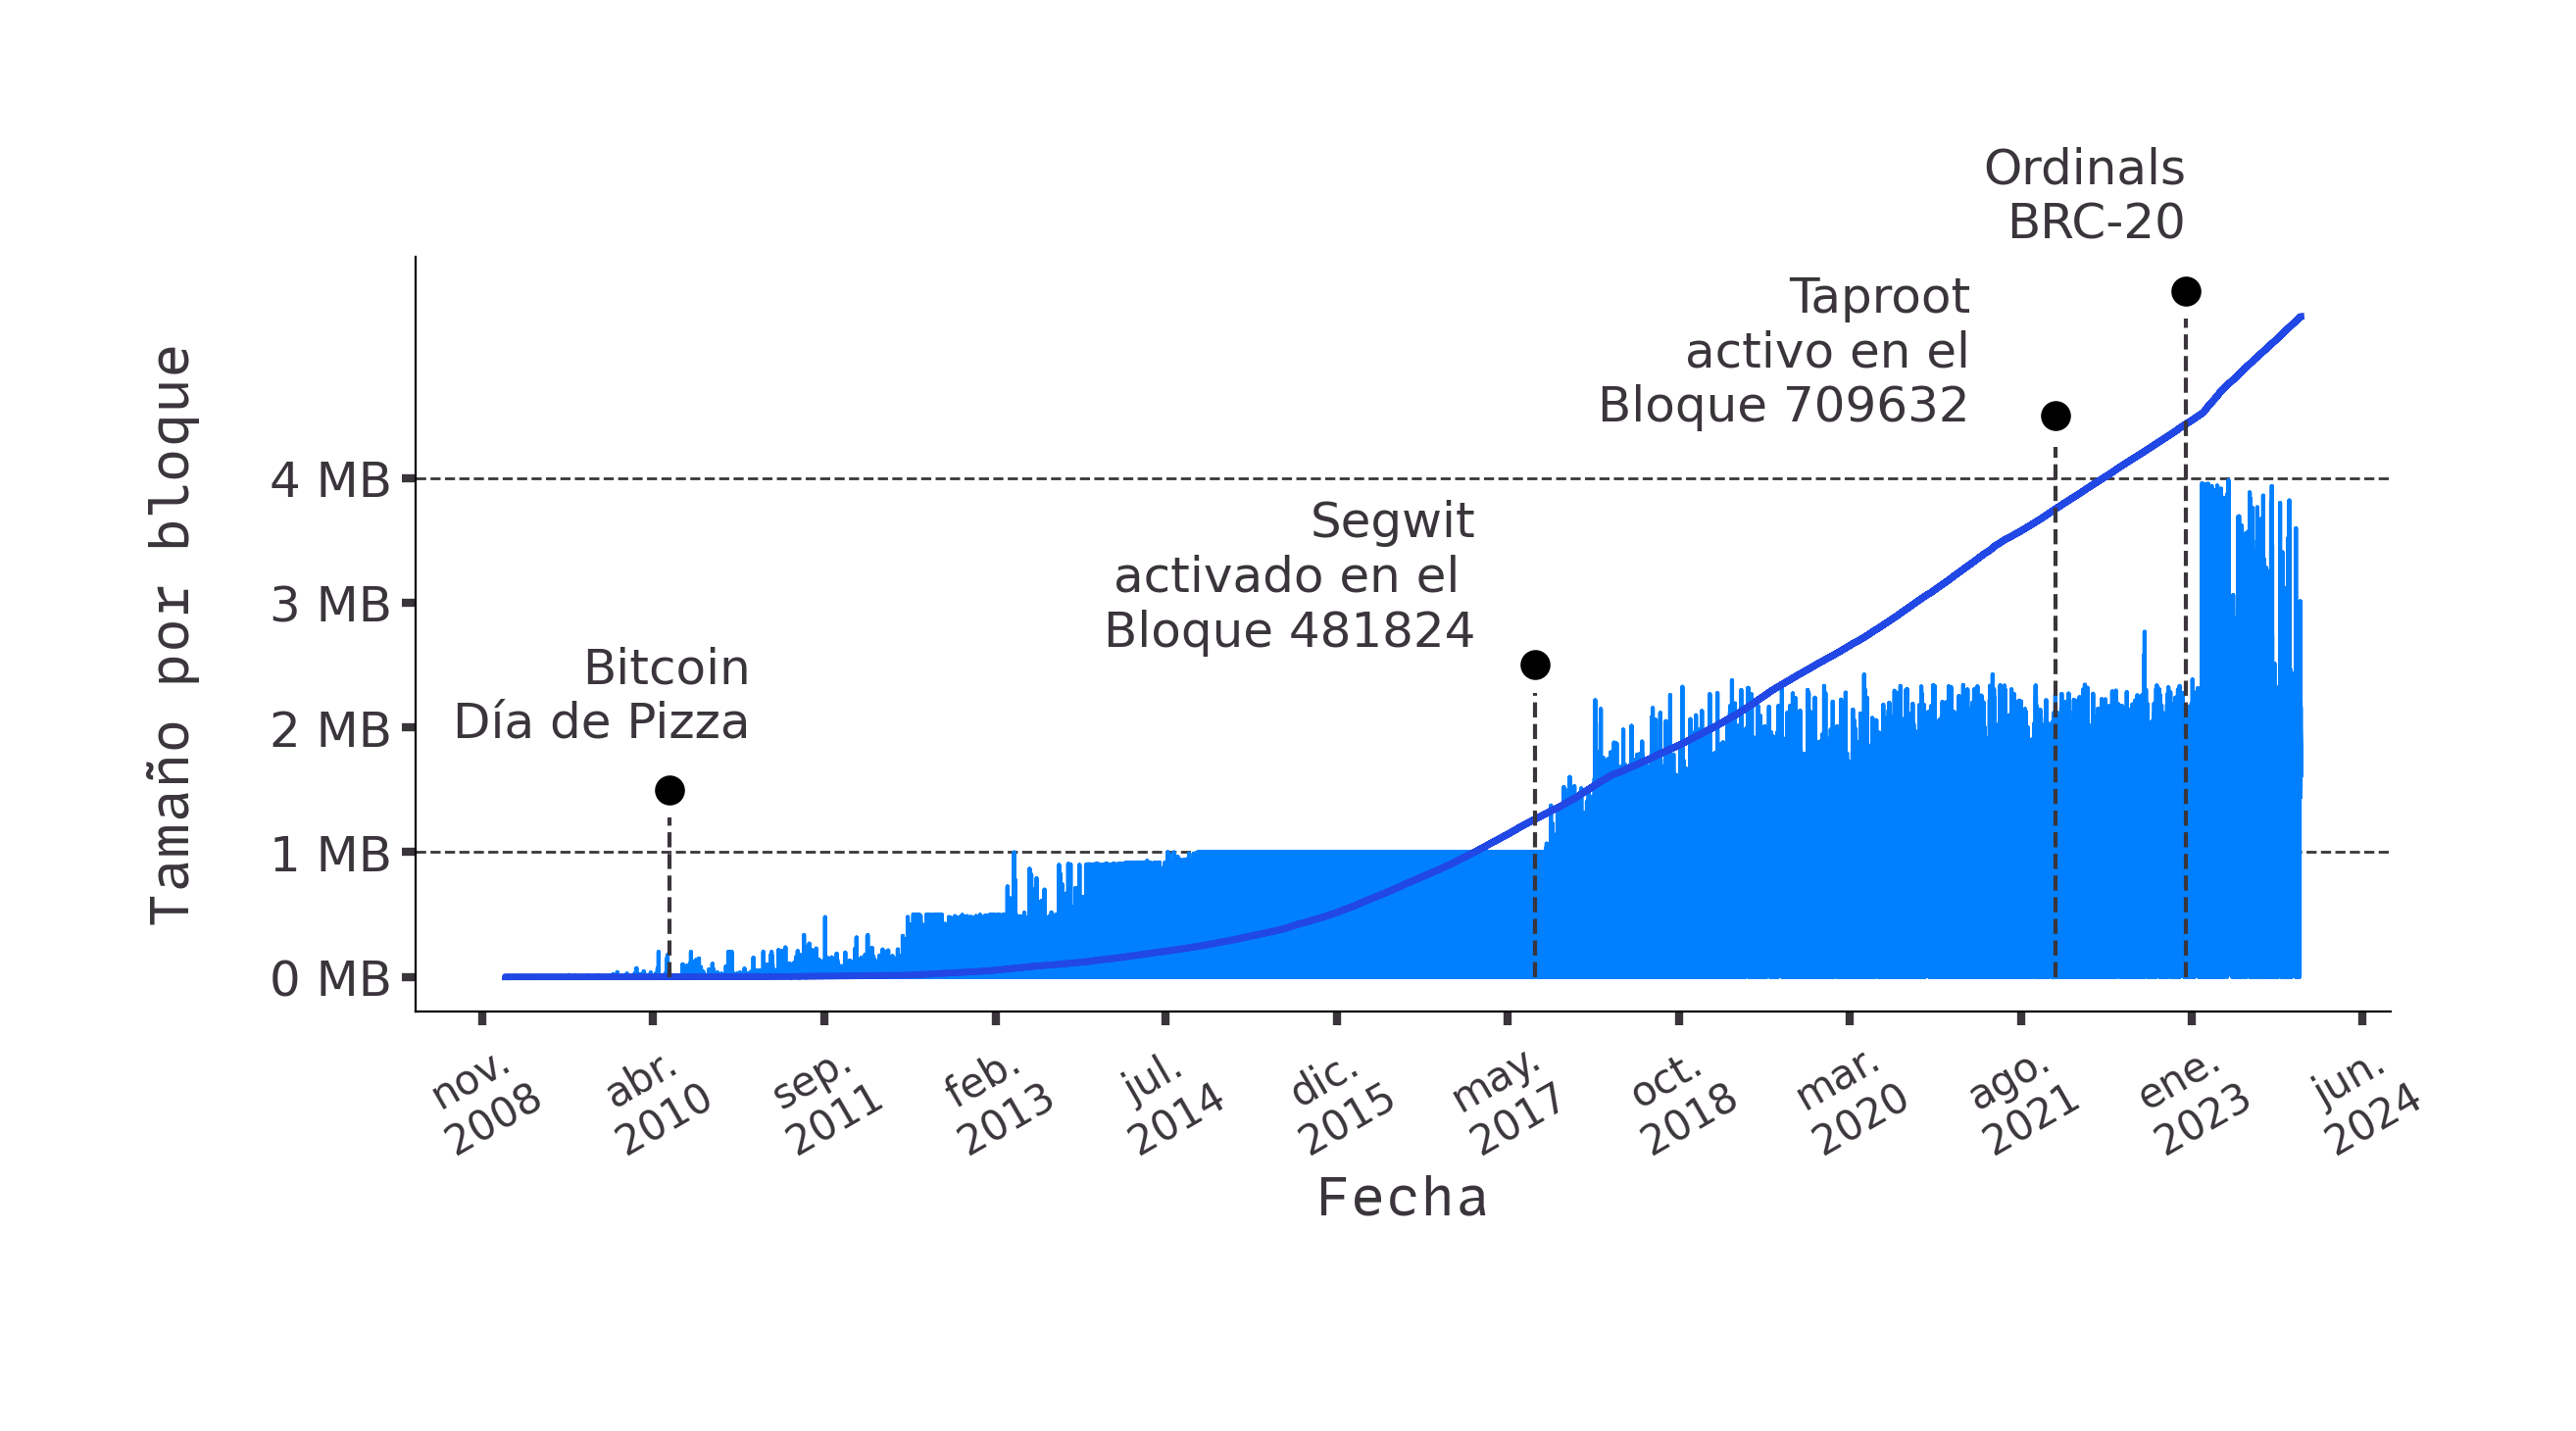
\includegraphics[width=0.6\textwidth]{blocksize_estilo_blanco.png}
    
 \caption{Tamaño en Bits por bloque desde el inicio de la red hasta el presente.- }
El día de la pizza se refiere al día en que un hombre pago con 10.000 bitcoin una pizza en ese tiempo valuados en 41 dolares.-
Segwit activate fue el día en que se hizo el Segregated Witness que fue una implementación de un soft fork (un cambio leve ) a la red con el fin de cambiar el formato de las transacciones en bitcoin.
Taproot fue una de las implementaciones mas significativas en la red y fue hecha con el fin de acelerar la verificación de las transacciones, durante su implementación conllevo a una especie de guerra civil entre los nodos que querían actualizar y aceptar esta implementación y los que no lo que llevo a la creación de Bitcoin Cash como otra moneda y como una nueva red.-
Ordinals BRC-20 fue la implementación de una idea, ya que las transacciones permiten almacenar información dentro de su Scritp Sig que es la parte de la transacción que contiene la información de la firma y es utilizado para la creación del UTXO, es posible usar este pequeño espacio para guardar información, entre los usos que le dieron están el guardar frases,pequeños poemas e incluso la información de los metadatos de NFT's (Non Fungible Token), esto significo un incremento en el tamaño de los bloques.

\end{figure}

\begin{figure} [h]
  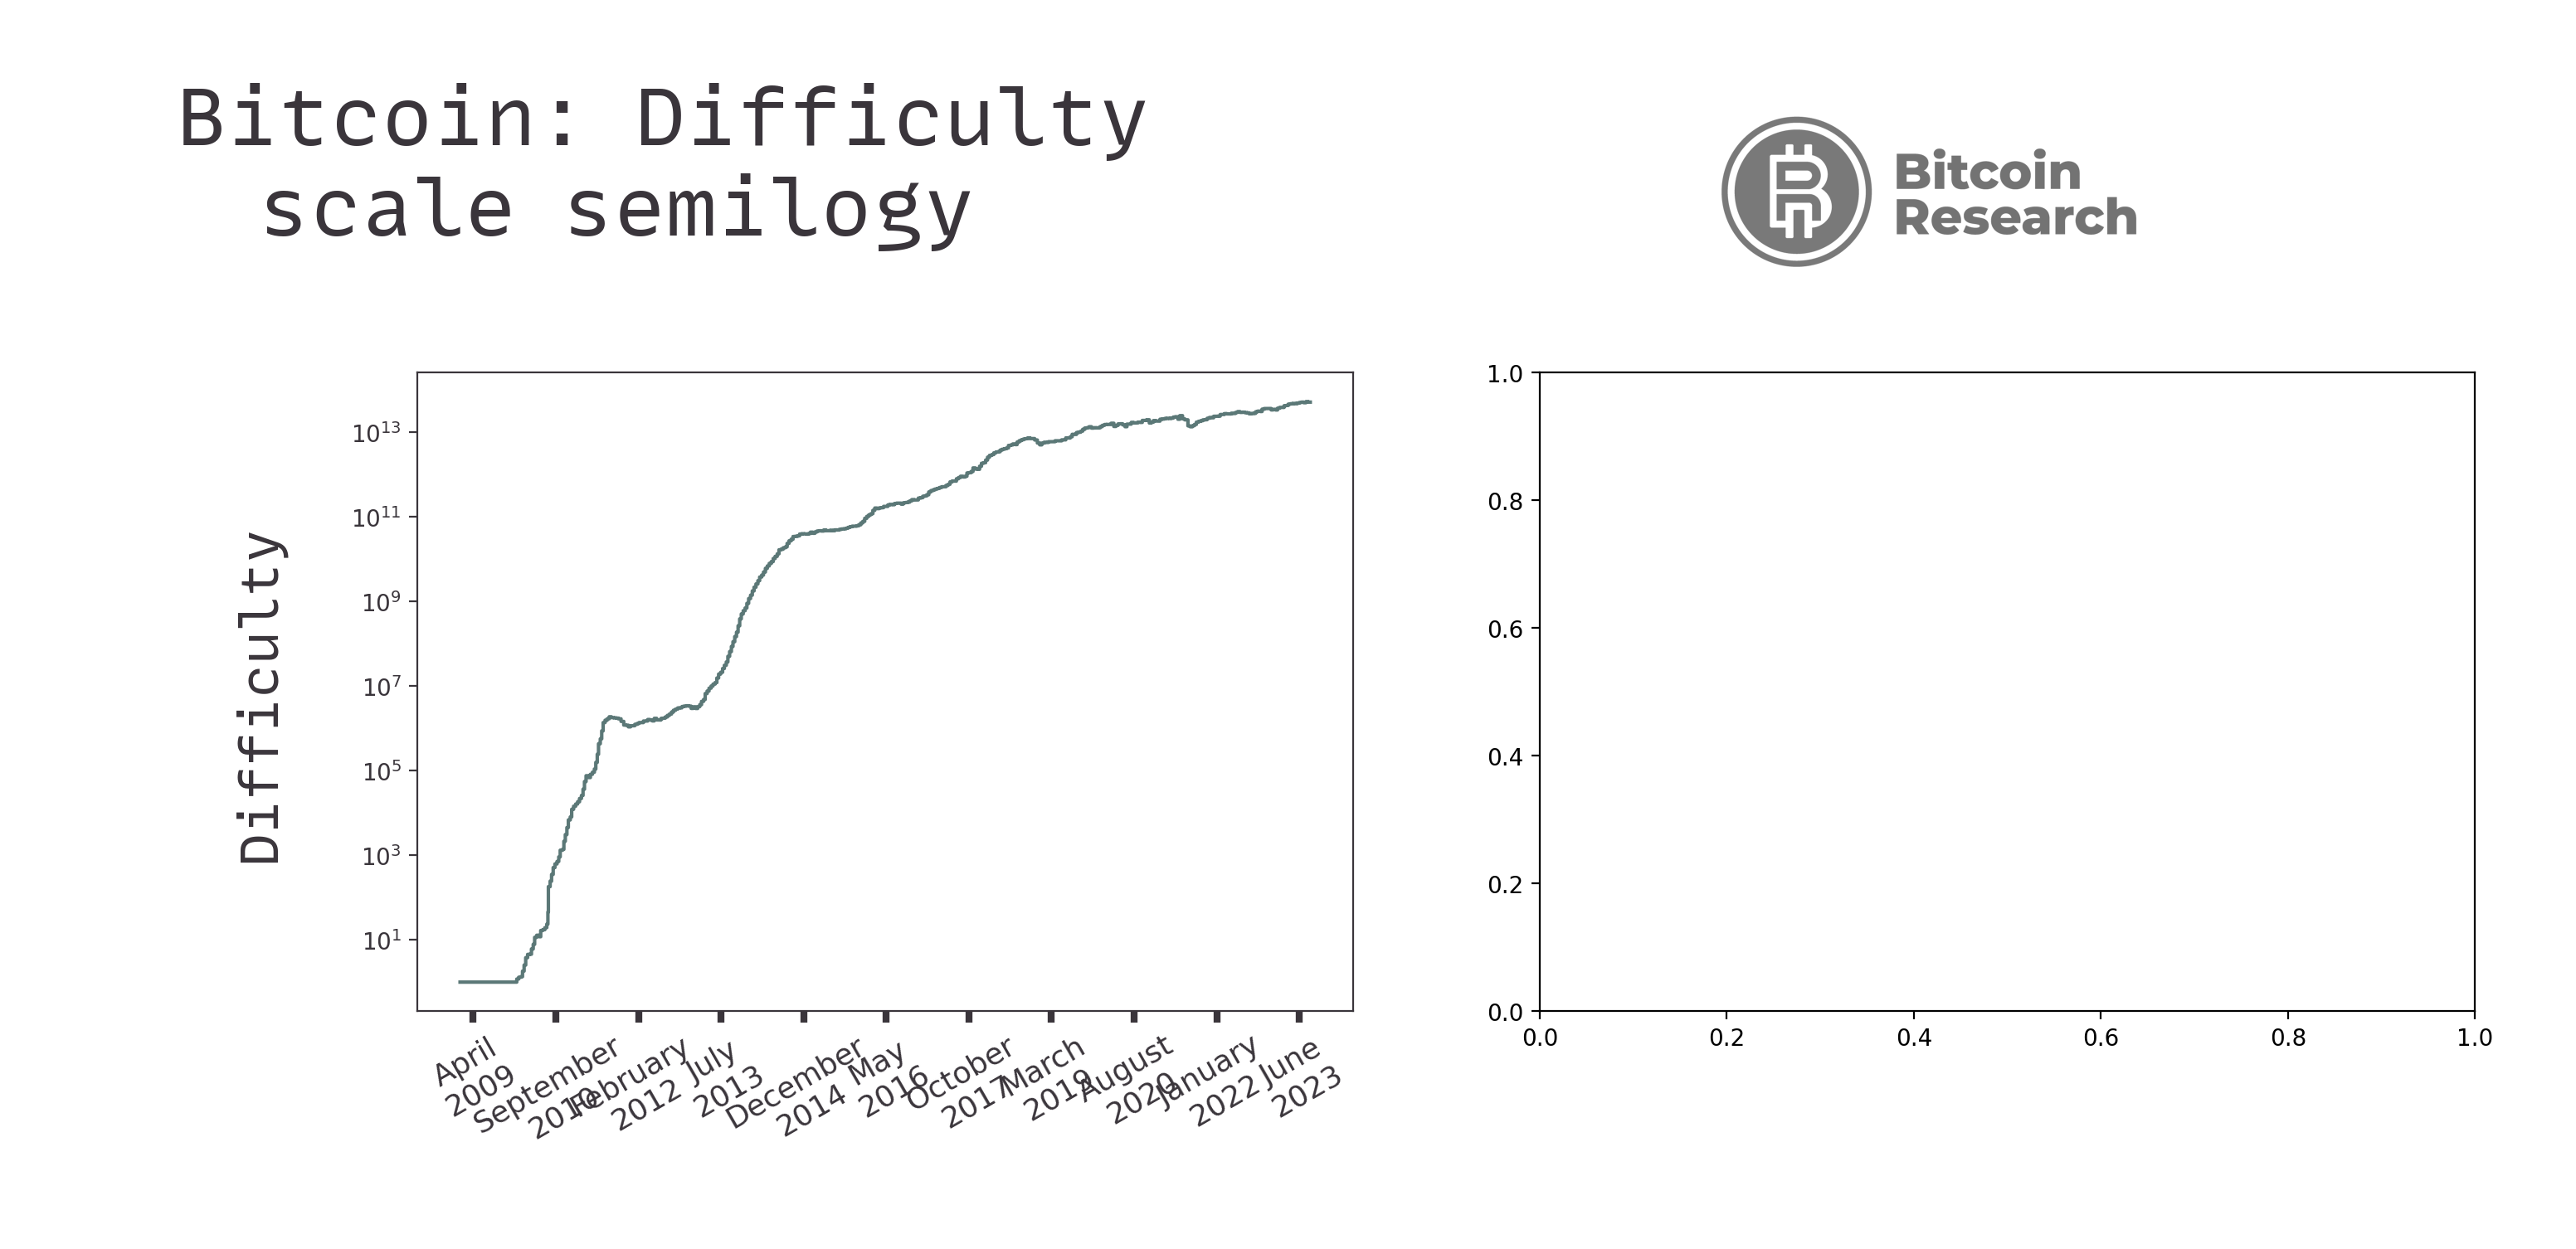
\includegraphics[width=0.5\textwidth]{dificultad_total_estilo_blanco.png}
    
 \caption{Evolución de la dificultad desde el inicio de la red.-Hasta el bloque 811298, el máximo histórico fue de 57,32 T hasta el 3 de octubre de 2023, además que la caída del tamaño de los bloques pudo ser causado por la prohibición de China del minado de criptomonedas esta acción fue llevada a cabo en agosto del 2021. }

\end{figure}


\begin{figure*} 
\centering
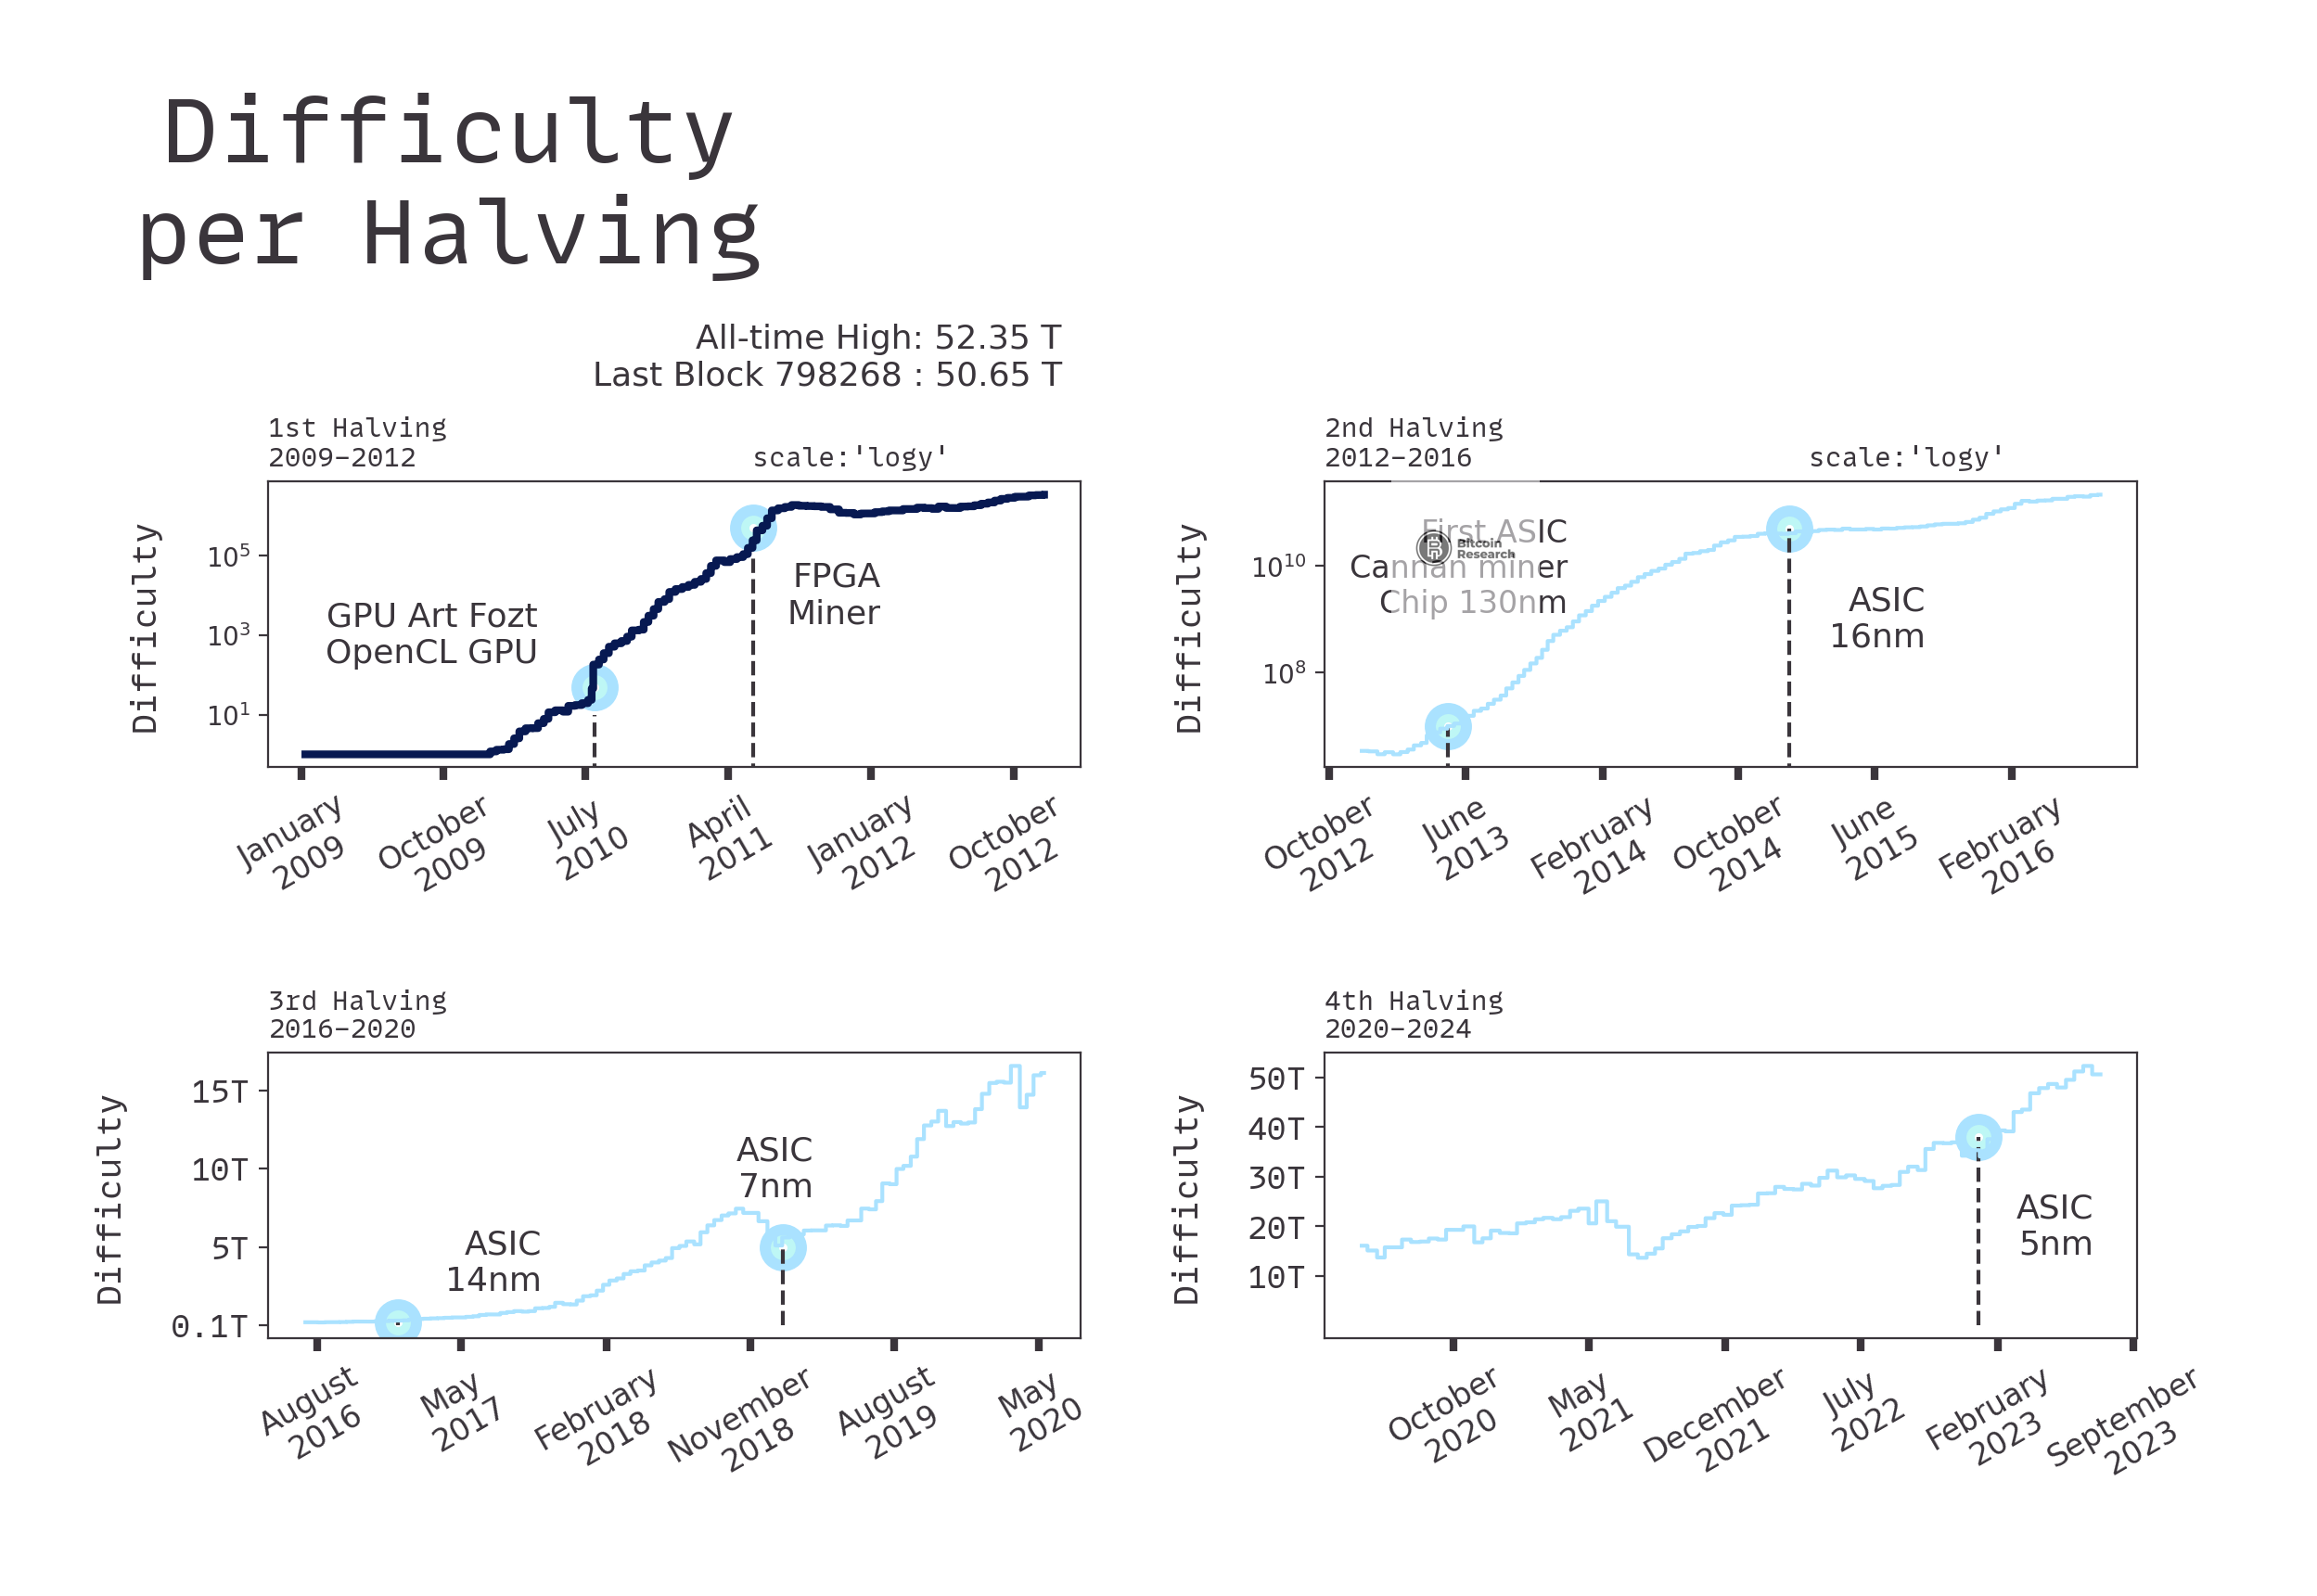
\includegraphics[width=1\textwidth]{dificultad_halv_estilo_blanco.png}
    
 \caption{Evolución de la dificultad por Halving.- GPU Art Fozt (Graphics Processing Unit) se refiere al uso de tarjetas gráficas domésticas, FPGA (Field Programmable Gate Arrays) se refiere a circuitos internos de matrices programables, y el término ASIC (Application-Specific Integrated Circuit) hace referencia a circuitos dedicados exclusivamente a la minería de criptomonedas. Desde su implementación, la mejora de estos dispositivos ha estado centrada en hacerlos más pequeños y mejorar su rendimiento para que consuman menos energía.  }

\end{figure*}


\begin{figure*} 
  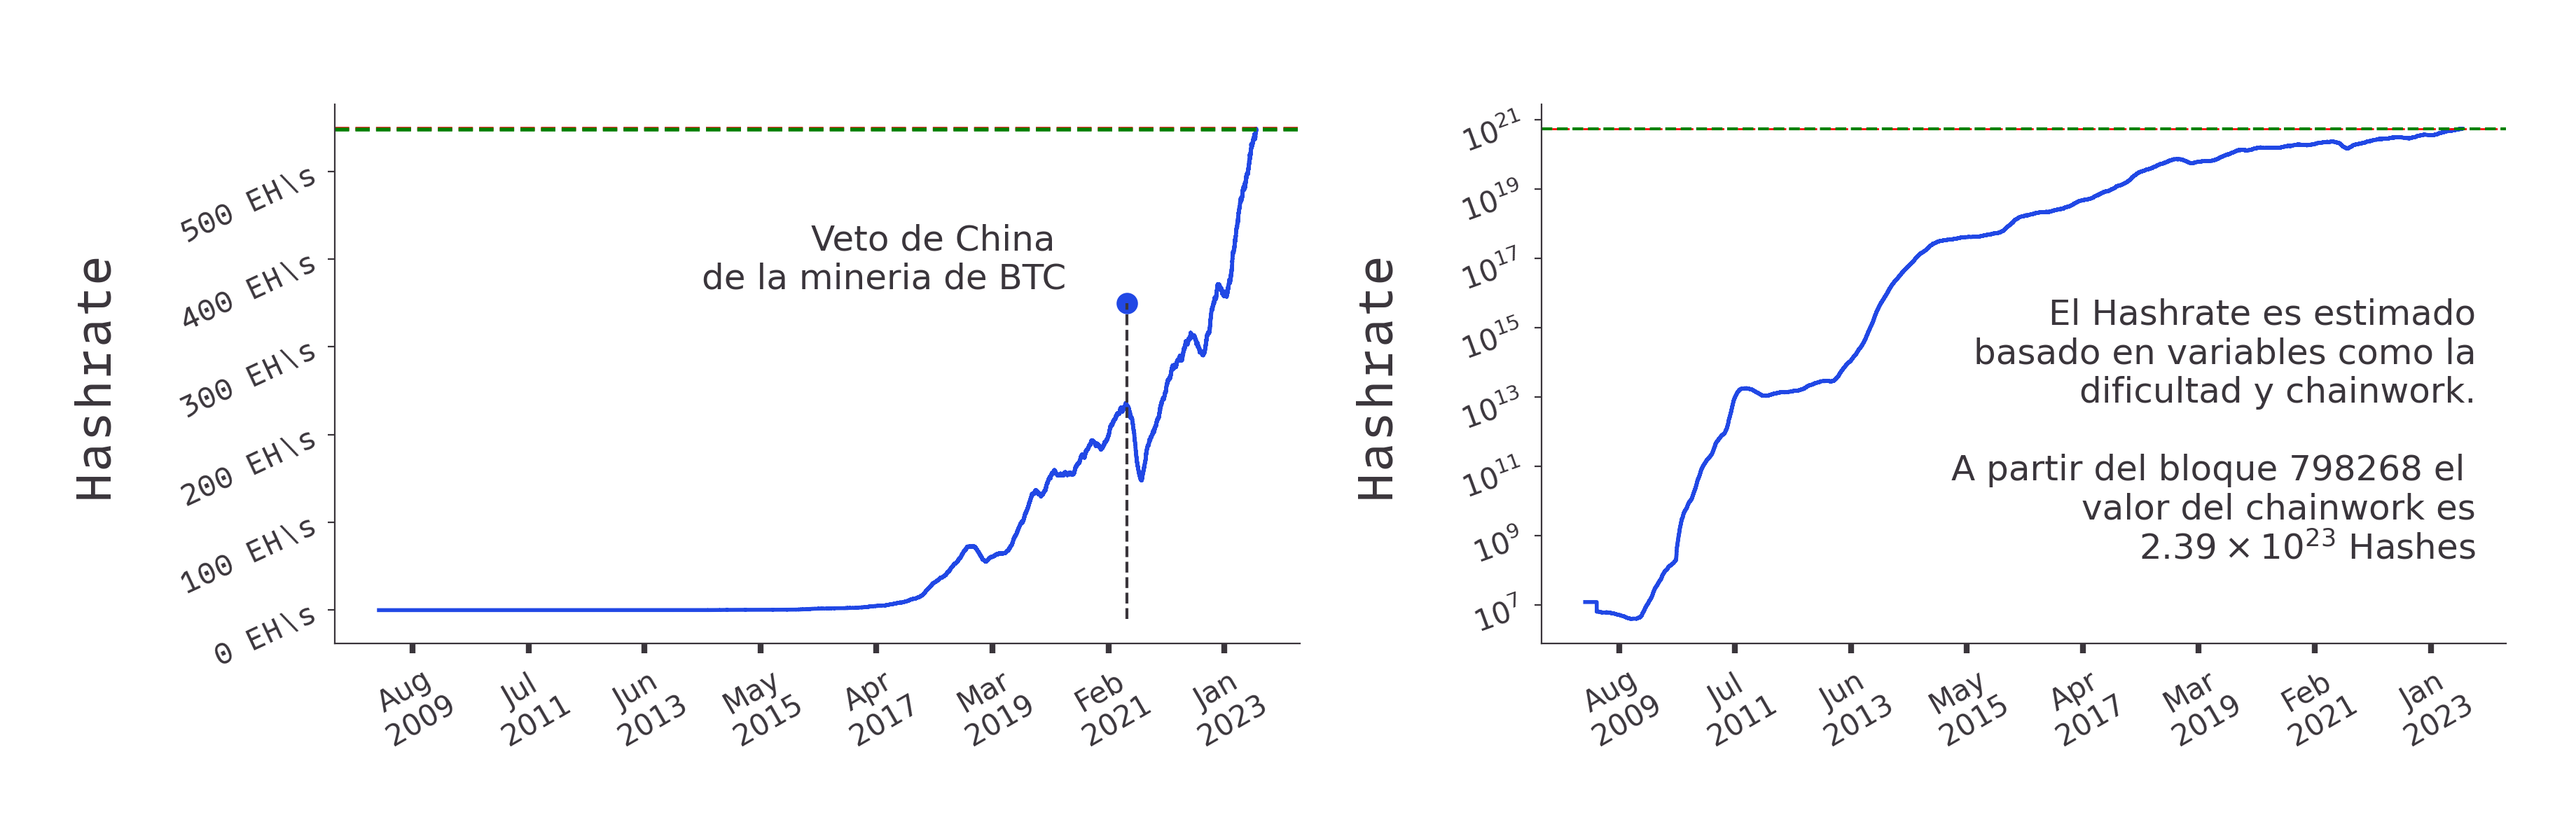
\includegraphics[width=1\textwidth]{hashrate_estilo_blanco.png}
    
 \caption{Tamaño en Bits por bloque desde el inicio de la red hasta el presente.-Hashrate es la cantidad de intentos que se llevaron a cabo para crear un hash que cumpla con los requisitos de complejidad exigidos por la red a través de la dificultad, estos valores son estimados a partir de los datos de la dificultad(la dificultad se mide en términos de hashes o intentos de hash por bloque) y el chainwork (cantidad de esfuerzo computacional empleado en la creación de los bloques dentro la red).    }
\end{figure*}



\begin{figure*} 
  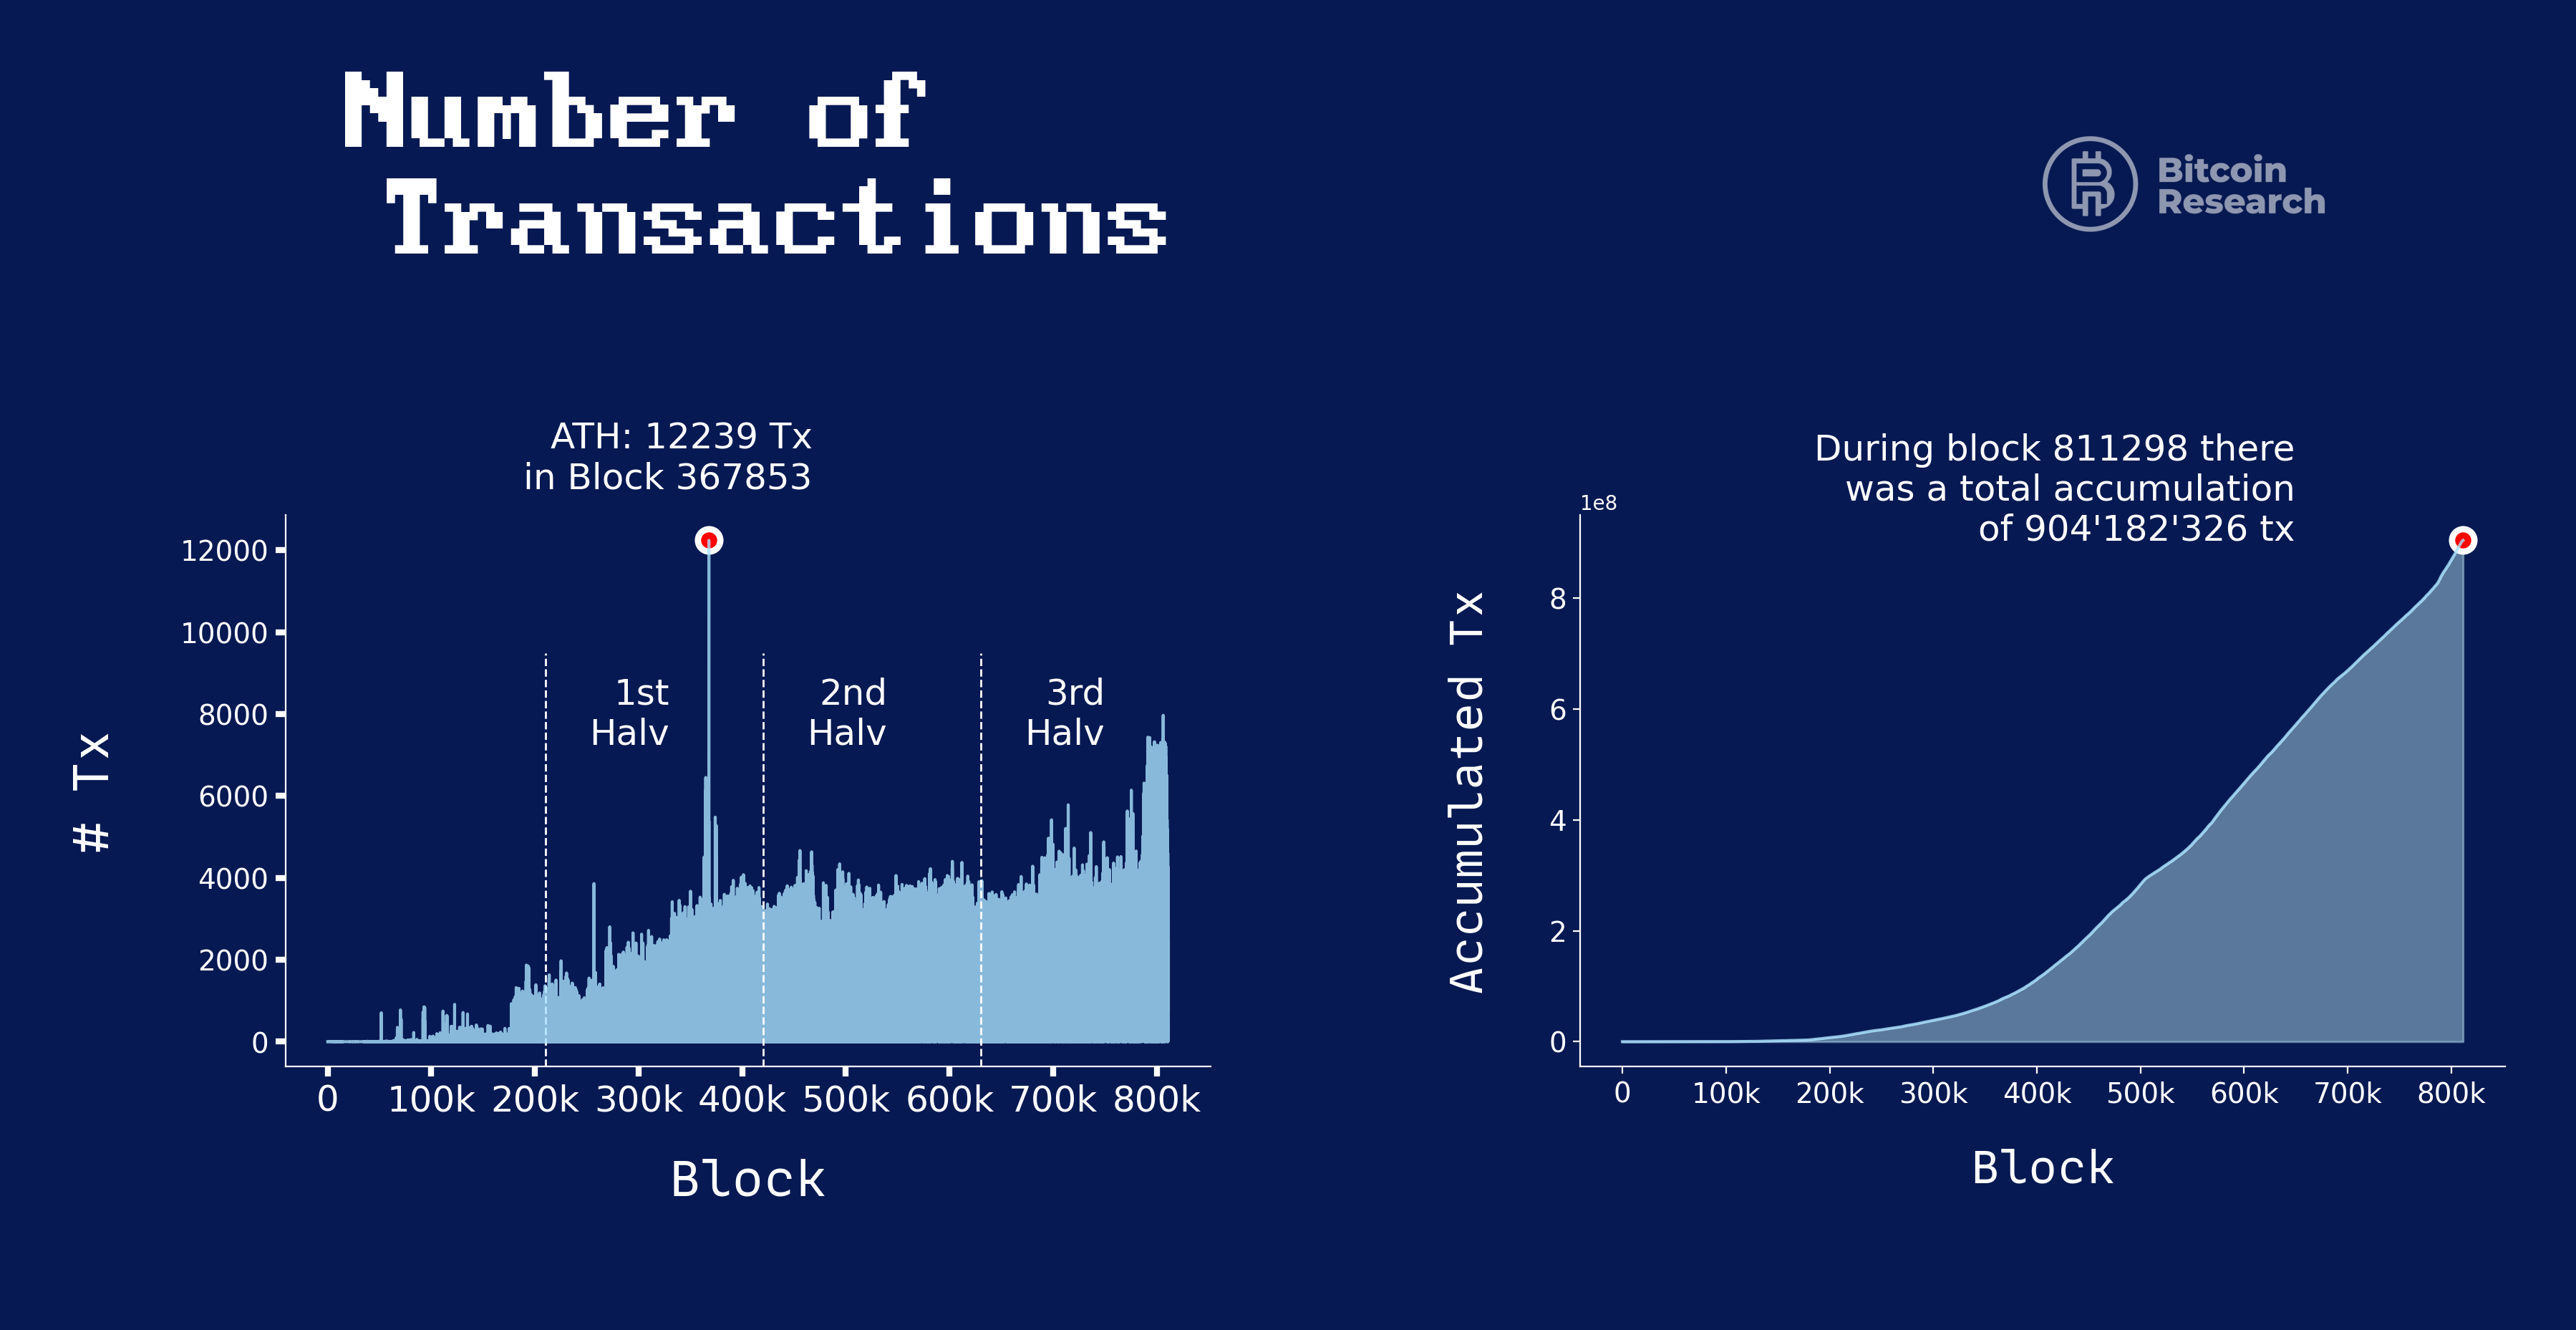
\includegraphics[width=1\textwidth]{Numero_de_transacciones_estilo_dark.png}
    
 \caption{Evolución del número de transacciones de cada bloque desde el inicio de la red-Se debe notar que el máximo histórico sucedió en el segundo halving la cantidad máxima de transacciones que puede tener un bloque esta condicionado a 1 MB de información- Acumulado del número de transacciones  }
 \end{figure*}


 
\begin{figure*} 
  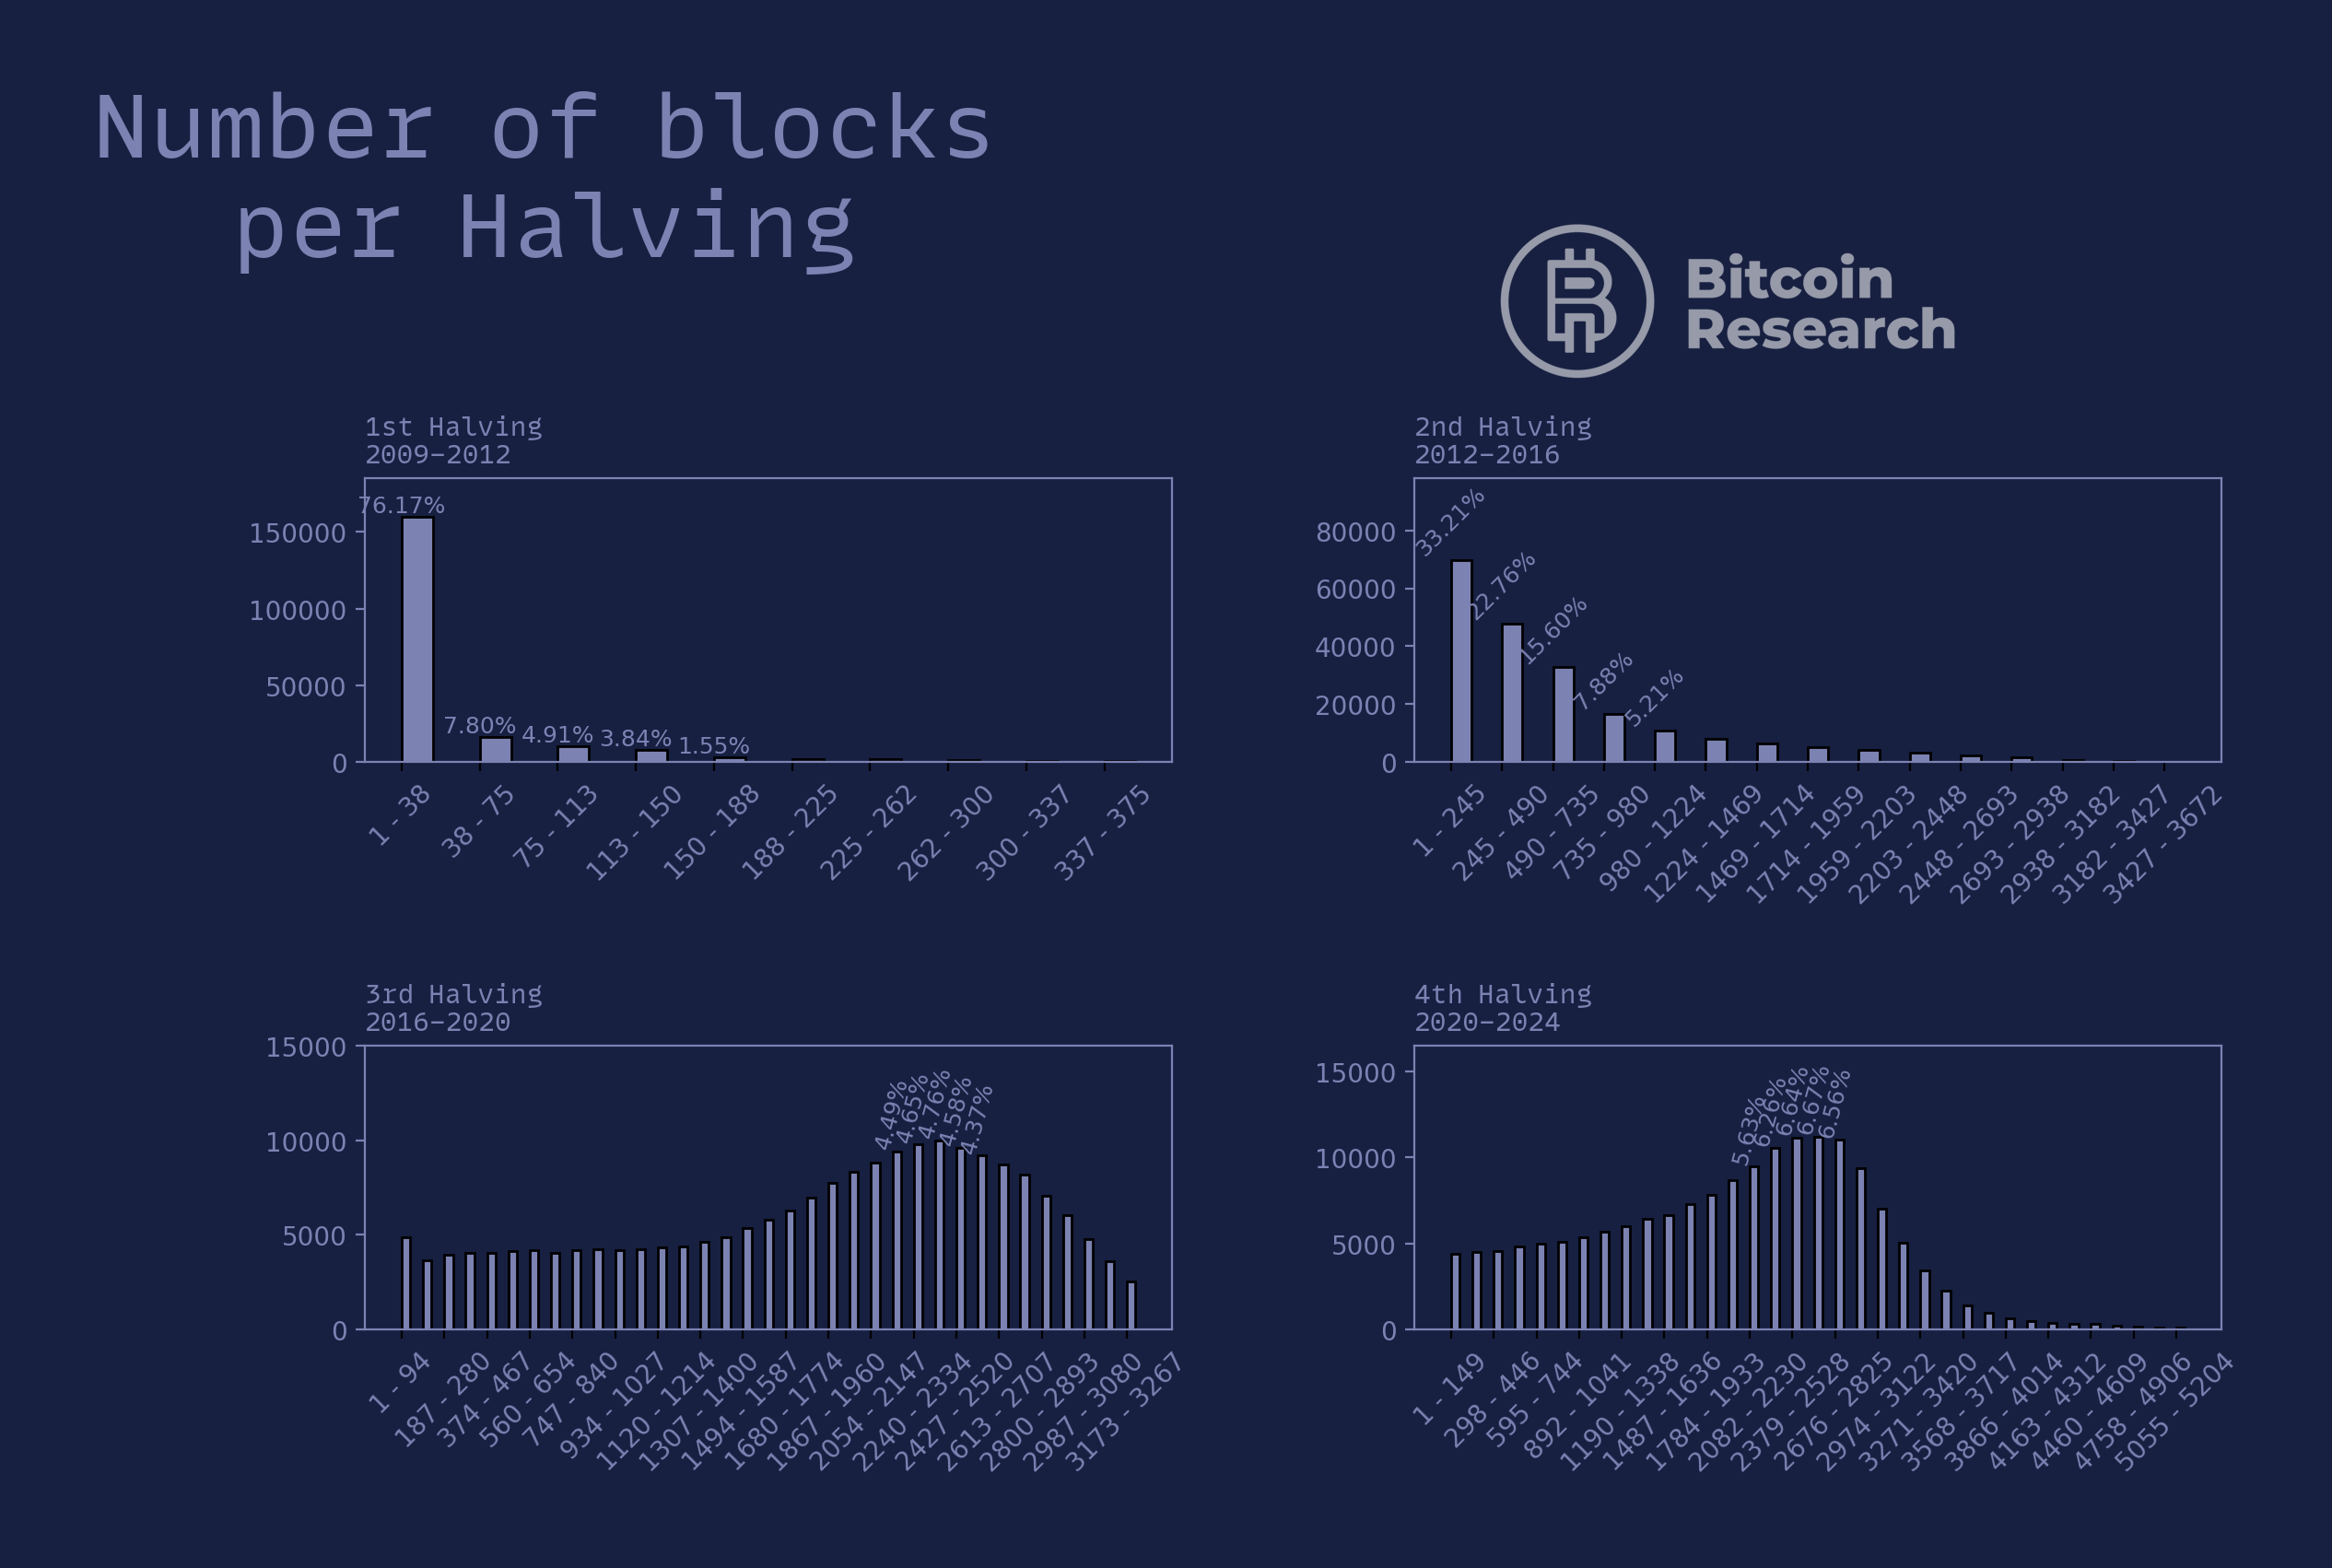
\includegraphics[width=1\textwidth]{Numero_de_transacciones_halv_estilo_dark.png}
    
 \caption{Número de Bloques contra número de transacciones en intervalos .-Al inicio de la red los bloques se subían con una transacción perteneciente al coinbase. El máximo histórico se sale de la gráfica, pero pertenece al segundo Halving }
\end{figure*}


\begin{figure*} 
  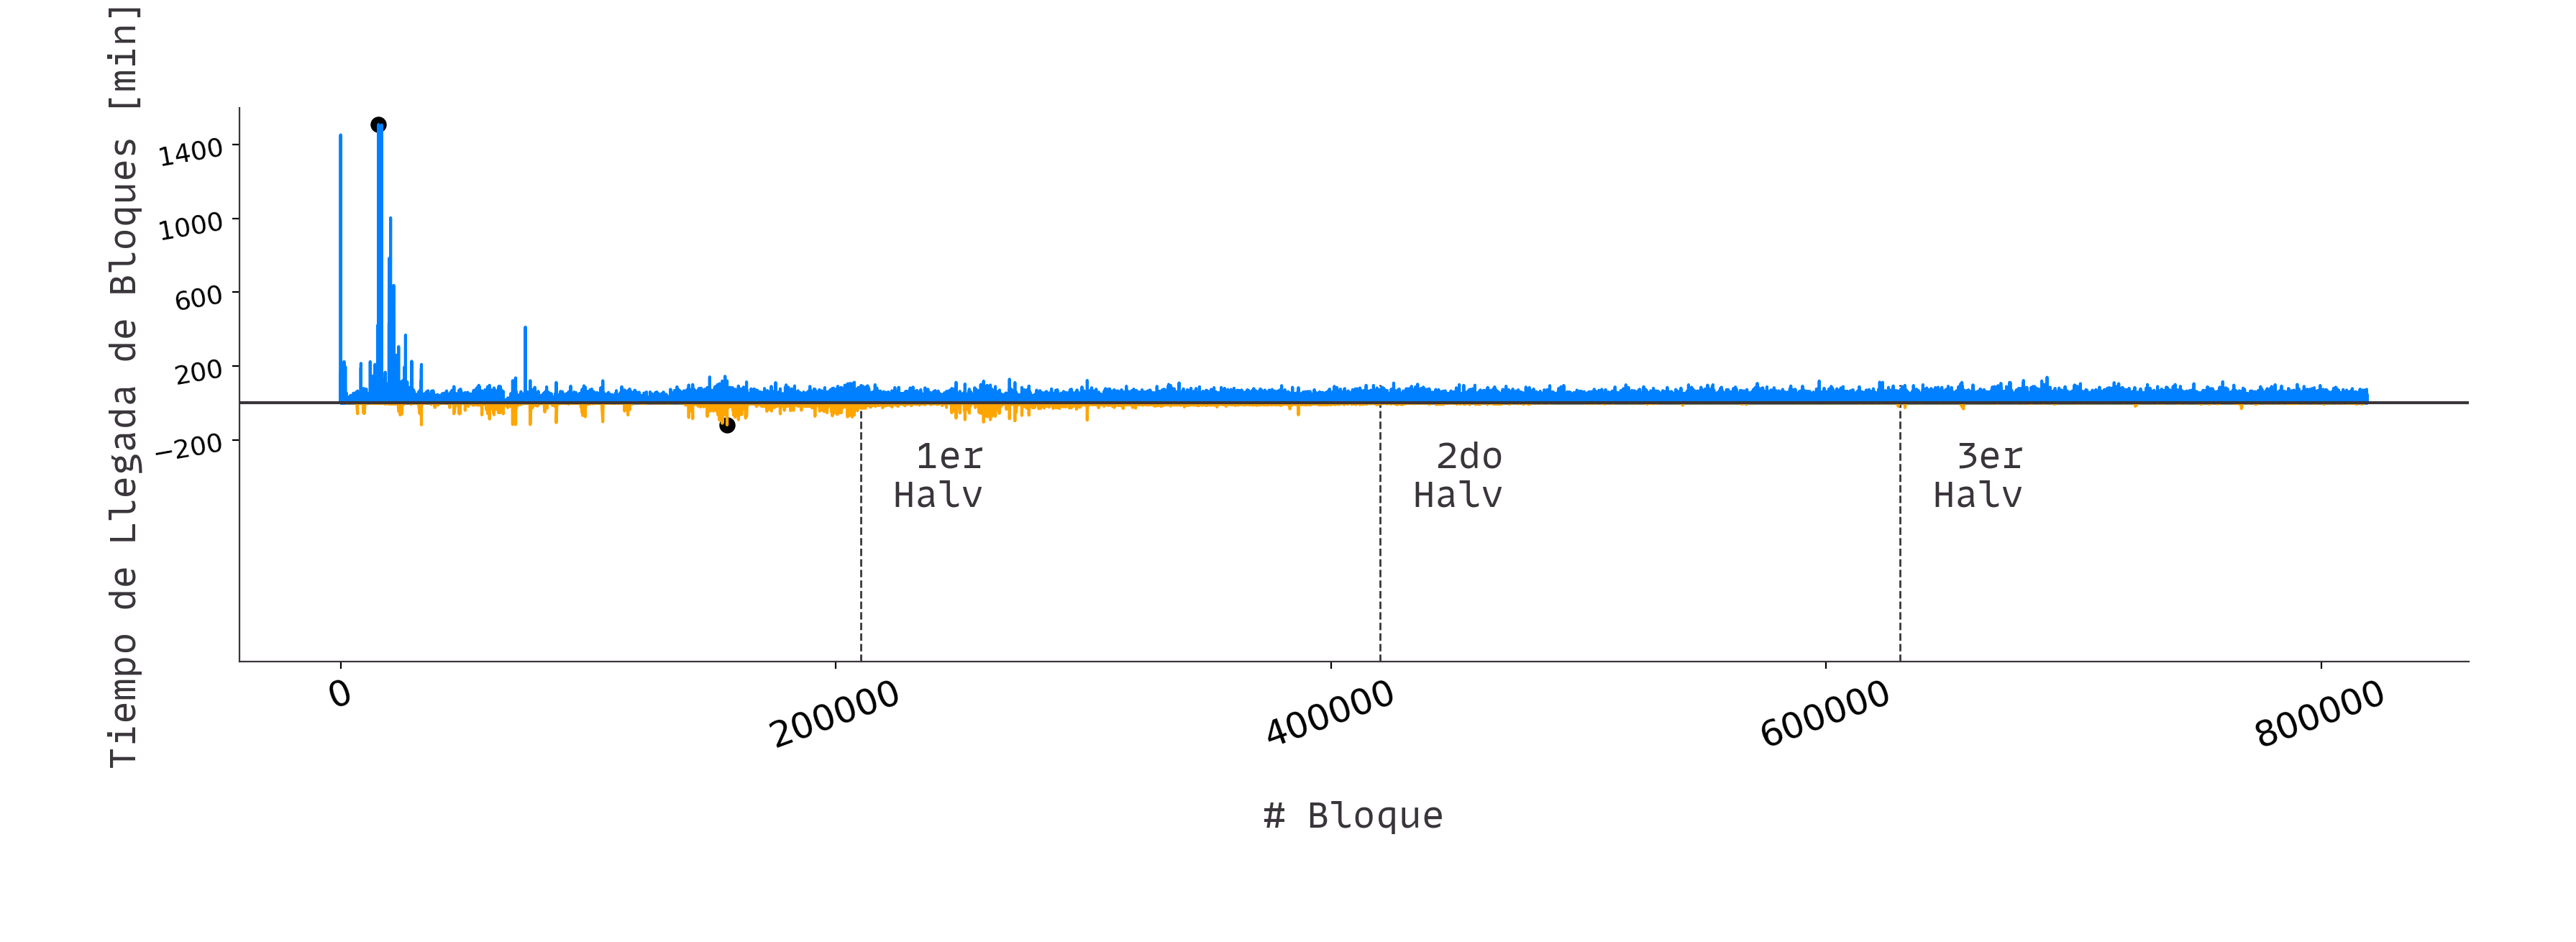
\includegraphics[width=1\textwidth]{timestamp_estilo_blanco.png}
    
 \caption{Tiempo de llegada de cada bloque Azul,Diferencia de tiempo entre el bloque y el siguiente.-Se debería esperar que los bloques lleguen con tiempos de llegada consecutivos pero existen bloques que se subieron con tiempos de llegada anteriores al de la red Naranja.-Estas anomalías temporales aparecen desde el primer Halving, pero suceden con menos frecuencia al día de hoy y su diferencia de tiempo es demasiado pequeña, su existencia puede estar ligada a momentos en que la red sufrió forks o incluso se reporto que algunos bloques podían ser subidos a la red de manera intencional con esta anomalía temporal }
\end{figure*}

\begin{figure*} 
  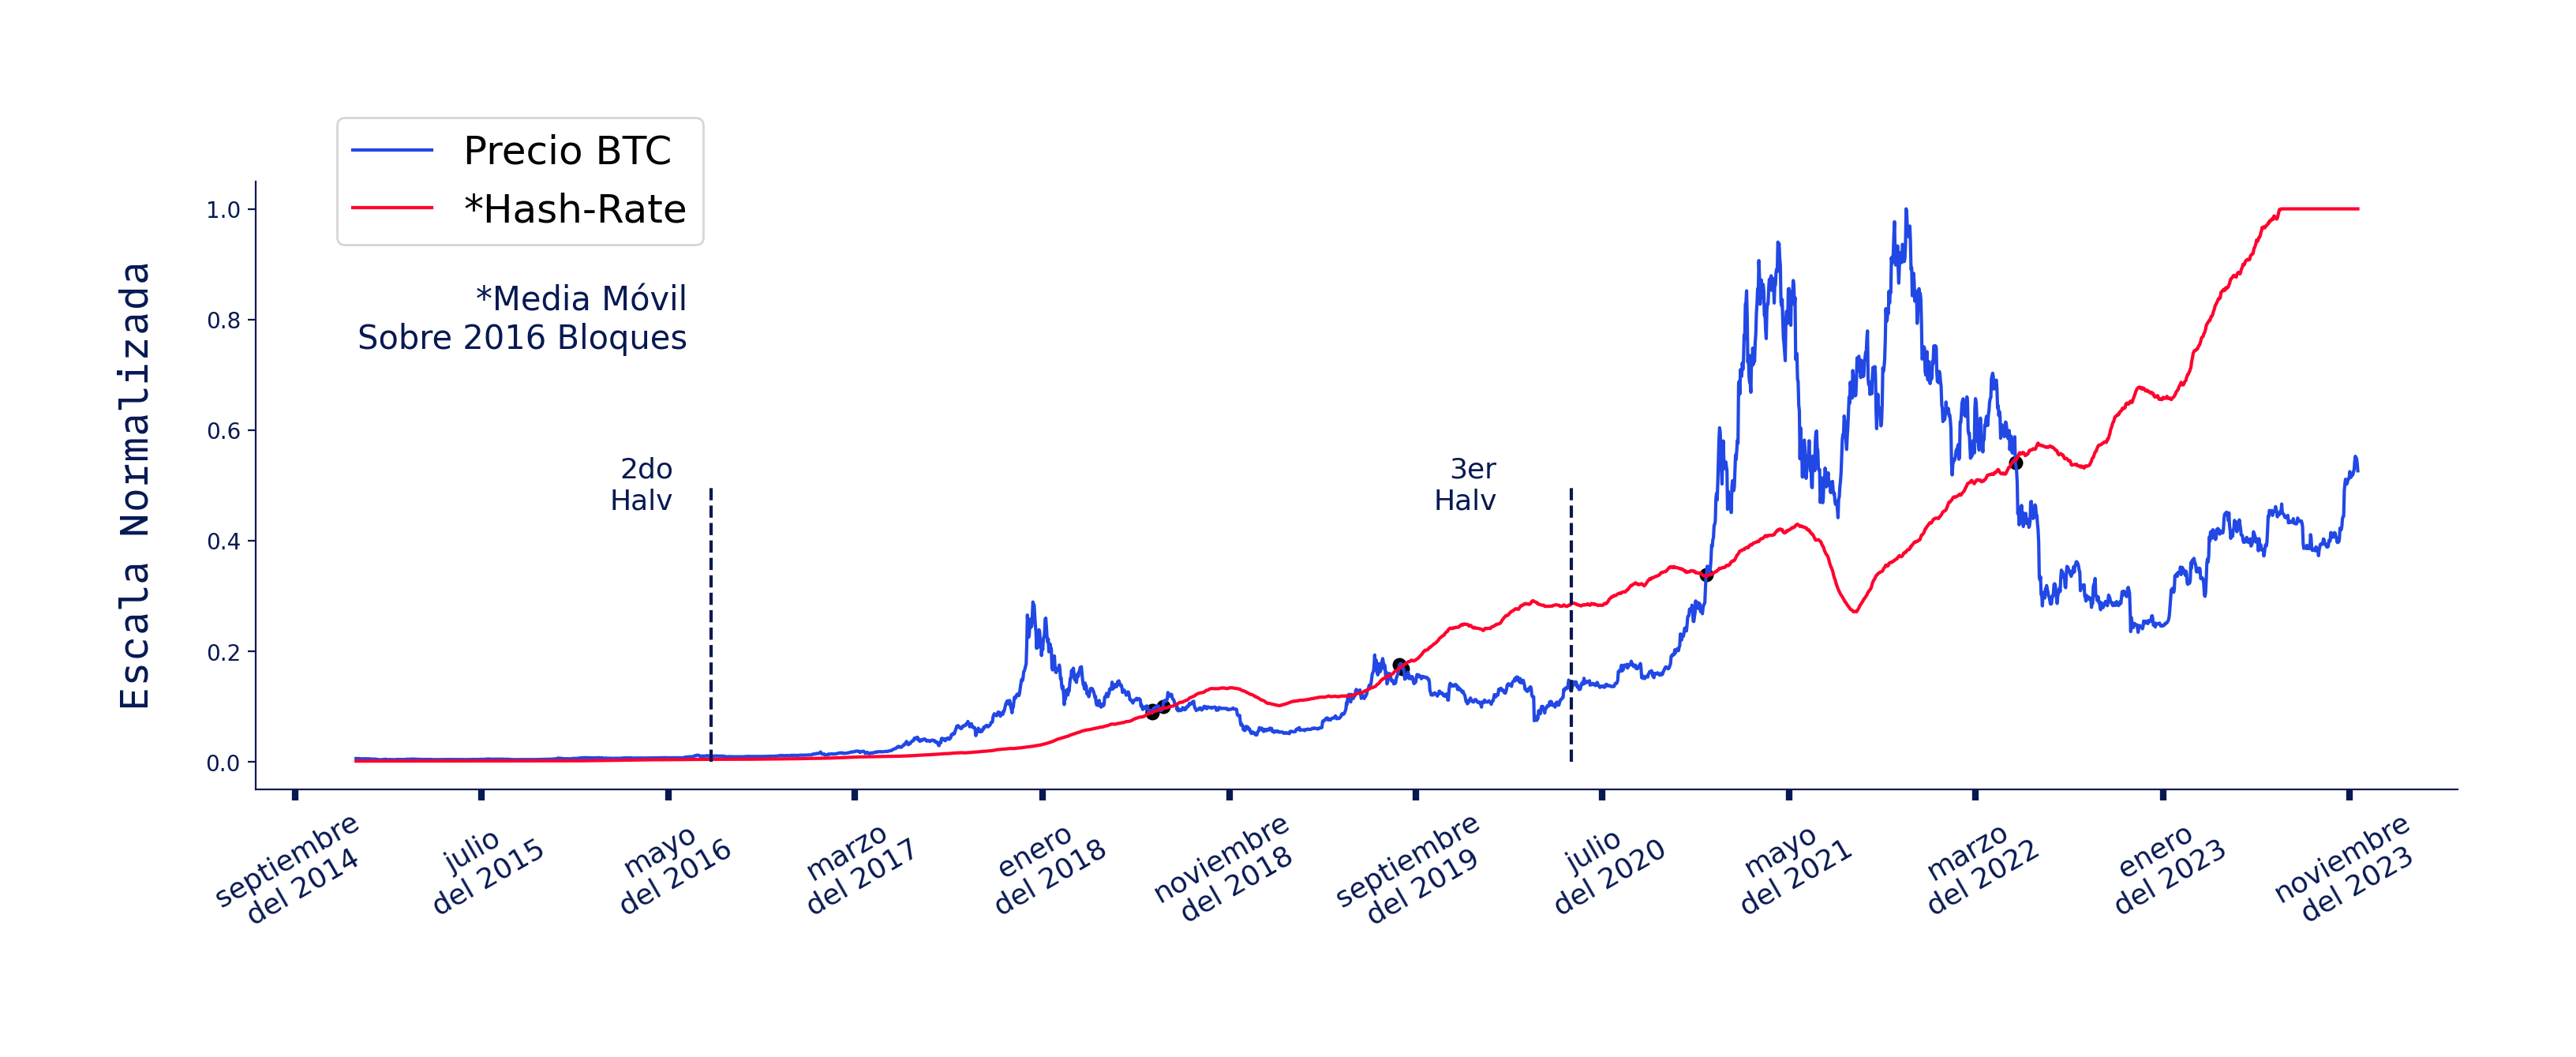
\includegraphics[width=1\textwidth]{pricHash_estilo_dark.png}
    
 \caption{Análisis histórico del precio de Bitcoin en dólares: la red de Bitcoin no proporciona datos sobre el precio de Bitcoin, ya que éste es externo y se define a través de la relación entre la oferta y la demanda. El hashrate es un factor crucial para determinar el precio, ya que un consumo excesivo de energía puede hacer que la minería de Bitcoin deje de ser rentable.  }
\end{figure*}
\section{Conclusiones}

\begin{thebibliography}

\bibitem[{Charles (1993)}] {charles}
Charles M.(1993), Revista de la Sociedad Española de Historia de las Ciencias y de las T{\'e}cnicas {\bf 16} 241

\bibitem[{Bielajew (2001)}] {biela}
Bielajew A. (2001), Some random thoughts on Monte Carlo electron and photon transport (Springer)



\end{thebibliography}


\end{document}